% Longitudinal MRI project report using the supplied AIDS LaTeX template.
% Main file: report.tex. Compile with XeLaTeX three times after a clean build.
\documentclass[12pt]{report}

% ---------------- Page setup (same as the Word file) -----------------
\usepackage[letterpaper,
            top=1.38in, bottom=1.18in, left=1.58in, right=1.18in,
            headsep=0.38in, footskip=0.5in]{geometry}

% ---------------- Fonts ----------------------------------------------
\usepackage{fontspec}
% Body: Times New Roman (falls back to a Times clone if not installed)
\IfFontExistsTF{Times New Roman}{\setmainfont{Times New Roman}}{%
  \IfFontExistsTF{TeX Gyre Termes}{\setmainfont{TeX Gyre Termes}}{%
    \setmainfont{Liberation Serif}}}
% Header / footer: Calibri (falls back to Carlito, its metric clone)
\IfFontExistsTF{Calibri}{\newfontfamily\hffont{Calibri}}{%
  \IfFontExistsTF{Carlito}{\newfontfamily\hffont{Carlito}}{%
    \newfontfamily\hffont{Liberation Sans}}}

% ---------------- Packages -------------------------------------------
\usepackage{graphicx}
\usepackage{xcolor}
\usepackage{setspace}
\usepackage{fancyhdr}
\usepackage{titlesec}
\usepackage{titletoc}
\usepackage{enumitem}
\usepackage{array}
\usepackage{booktabs}
\usepackage[labelsep=colon]{caption}
\usepackage[numbers,square,sort&compress]{natbib}
\usepackage[hidelinks]{hyperref}   % clickable TOC entries, no coloured boxes

\definecolor{wordred}{HTML}{FF0000}
\newcommand{\red}[1]{\textcolor{wordred}{#1}}

\setlength{\parindent}{0pt}
\setlength{\parskip}{6pt}

% =====================================================================
%  EDIT THESE DETAILS
% =====================================================================
\newcommand{\projecttitle}{World Models for Longitudinal Glioma MRI}
\newcommand{\monthyear}{November 2026}       % header (right) and title page
\newcommand{\guidename}{Dr. Manju Venugopalan, Assistant Professor (Selection Grade)}

% ---------------- Headers and footers --------------------------------
% Front matter: centred roman page number only
\fancypagestyle{front}{%
  \fancyhf{}
  \renewcommand{\headrulewidth}{0pt}
  \fancyfoot[C]{\thepage}}

% Main chapters: CURRENT CHAPTER NAME (left, automatic) | Month, year (right)
% Footer: Dept. of CSE, ASC, Bengaluru (left) | Page | n (right)
\fancypagestyle{main}{%
  \fancyhf{}
  \renewcommand{\headrulewidth}{0pt}
  \fancyhead[L]{\hffont\small\leftmark}
  \fancyhead[R]{\hffont\small\monthyear}
  \fancyfoot[L]{\hffont\small\vspace*{\baselineskip}Dept. of CSE, ASAI, Bengaluru}
  \fancyfoot[R]{\hffont\small Page | \thepage\vspace*{\baselineskip}}}
\fancypagestyle{plain}{}          % chapter pages keep the same header

\renewcommand{\chaptermark}[1]{\markboth{#1}{}}   % header = chapter title
\renewcommand{\sectionmark}[1]{}

% \chapter does NOT start a new page by itself (so notes can sit above
% the heading). Put \clearpage before every \chapter.
\makeatletter
\renewcommand{\chapter}{\global\@topnum\z@\@afterindentfalse
  \secdef\@chapter\@schapter}
\makeatother

% ---------------- Headings -------------------------------------------
% Chapter:  "CHAPTER - n"  and the title below, centred, bold, 14 pt
\titleformat{\chapter}[display]
  {\normalfont\fontsize{14}{17}\bfseries\centering}
  {CHAPTER - \thechapter}{6pt}{\MakeUppercase}
\titlespacing*{\chapter}{0pt}{0pt}{18pt}
% Section 1.1 (bold 12 pt), Subsection 1.1.1 (bold 12 pt)
\titleformat{\section}{\normalfont\fontsize{12}{14}\bfseries}{\thesection}{0.6em}{}
\titlespacing*{\section}{0pt}{12pt}{6pt}
\titleformat{\subsection}{\normalfont\fontsize{12}{14}\bfseries}{\thesubsection}{0.6em}{}
\titlespacing*{\subsection}{0pt}{10pt}{4pt}

\setcounter{secnumdepth}{3}
\setcounter{tocdepth}{2}          % TOC shows chapters, sections, subsections

% ---------------- Table of Contents style ----------------------------
\contentsmargin{0.5in}
\newcommand{\tocdots}{\titlerule*[0.6pc]{.}}
% Chapters: "CHAPTER 1 – INTRODUCTION ........ 1"
\titlecontents{chapter}[0pt]{\addvspace{3pt}}
  {CHAPTER \thecontentslabel\ -- \MakeUppercase}
  {\hspace*{0.25in}\MakeUppercase}            % un-numbered entries
  {\tocdots\contentspage}
% Sections: "1.1 INTRODUCTION TO ....... 2"
\titlecontents{section}[0.95in]{}
  {\contentslabel{0.45in}\MakeUppercase}{\MakeUppercase}
  {\tocdots\contentspage}
% Subsections: "5.2.1 ..........  4"
\titlecontents{subsection}[1.55in]{}
  {\contentslabel{0.6in}\MakeUppercase}{\MakeUppercase}
  {\tocdots\contentspage}
% Figures and tables: "1.1   Role hierarchy ........ 5"
\titlecontents{figure}[0.55in]{\addvspace{2pt}}
  {\contentslabel{0.55in}}{}{\tocdots\contentspage}
\titlecontents{table}[0.55in]{\addvspace{2pt}}
  {\contentslabel{0.55in}}{}{\tocdots\contentspage}

\renewcommand{\contentsname}{TABLE OF CONTENTS}
\renewcommand{\listfigurename}{List Of Figures}
\renewcommand{\listtablename}{List Of Tables}
\renewcommand{\bibname}{REFERENCES}

% ---------------- Captions -------------------------------------------
% Figures: "Fig. 1.1: Title" below the figure; Tables: "Table 1.1: Title" above
\captionsetup[figure]{name=Fig., font=bf, labelfont=bf, skip=6pt}
\captionsetup[table]{name=Table, font=bf, labelfont=bf, position=top, skip=6pt}

% ---------------- References (IEEE style numbering "[1].") -----------
\renewcommand{\bibnumfmt}[1]{[#1].}
\setlength{\bibsep}{2pt}
\renewcommand{\bibpreamble}{}


\usepackage{longtable}
\usepackage{float}
\usepackage[section]{placeins}
\usepackage{microtype}
\setlength{\headheight}{14pt}
\setlength{\emergencystretch}{2em}
\renewcommand{\topfraction}{0.85}
\renewcommand{\bottomfraction}{0.75}
\renewcommand{\textfraction}{0.10}
\renewcommand{\floatpagefraction}{0.65}
\newcommand{\frontchapter}[1]{\clearpage\phantomsection\addcontentsline{toc}{chapter}{#1}\chapter*{#1}}

\begin{document}\addtocontents{toc}{\protect\hfill\textbf{Page No.}\protect\par}
\begin{titlepage}
\centering
\vspace*{0.6in}
{\fontsize{14}{17}\selectfont\bfseries \projecttitle\par}
\vspace{10pt}
A PROJECT REPORT\par
\vspace{10pt}
{\fontsize{14}{17}\selectfont\bfseries\itshape Submitted by\par}
\vspace{14pt}
\begin{tabular}{@{}l@{\hspace{0.45in}}l@{}}
BL.EN.U4AID23002 & Adithya Nair\\[16pt]
BL.EN.U4AID23005 & Avighna Reddy Katipally\\
\end{tabular}\par
\vspace{18pt}
{\fontsize{14}{17}\selectfont\bfseries\itshape in partial fulfillment for the award of the degree of\par}
\vspace{18pt}
{\fontsize{14}{17}\selectfont\bfseries BACHELOR OF TECHNOLOGY\par}
\vspace{16pt}
{\small IN\par}
\vspace{16pt}
ARTIFICIAL INTELLIGENCE AND DATA SCIENCE\par
\vspace{12pt}

\includegraphics[width=1.75in]{amrita_logo.png}\par
\vspace{12pt}
AMRITA SCHOOL OF ARTIFICIAL INTELLIGENCE, BENGALURU\par
\vspace{12pt}
{\fontsize{14}{17}\selectfont AMRITA VISHWA VIDYAPEETHAM\par}
\vspace{12pt}
BENGALURU 560 035\par
\vspace{12pt}
\MakeUppercase{\monthyear}\par
\end{titlepage}
\pagestyle{front}\pagenumbering{roman}\setcounter{page}{1}
\frontchapter{ACKNOWLEDGEMENTS}\begin{spacing}{1.5}\setlength{\parindent}{0.5in}
We thank everyone whose guidance and encouragement supported this project.

We offer our sincere pranams at the lotus feet of “AMMA”, MATA AMRITANANDAMAYI  DEVI who showered her blessing upon us throughout the course of this project work.

We owe our gratitude to Prof. Manoj P., Director, Amrita Vishwa Vidyapeetham Bengaluru Campus. We would like to place our heartfelt gratitude to Dr. Gopalakrishnan E.A., Principal, Amrita School of Computing and Amrita School of Artificial Intelligence, Bengaluru for his valuable support and inspiration.

We express our gratitude to our project guide, Dr. Manju Venugopalan, Assistant Professor (Selection Grade), Department of Computer Science and Engineering, Amrita School of Computing, Bengaluru, for her guidance and encouragement throughout the project.

We thank the project panel members for their suggestions and encouragement, the faculty for their academic support, and our parents for their continued support.
\end{spacing}
\frontchapter{ABSTRACT}\begin{spacing}{1.5}
  This study examines anatomical state estimation and prediction for longitudinal glioma MRI. We test methods across three data sets: LUMIERE  as the main set, SAILOR to evaluate transfer data, and MU-Glioma-Post for postoperative masks to evaluate a specific capability of our methods. Following glioma patient development over time requires more than simple MRI scans that are learned in isolation. A good signal for glioma development is understanding how anatomy changes over time. The motivating question is whether we can build a useful representation of the patient's current anatomy and does adding the history of the patient make the representation richer for predicting future anatomy. For current anatomy estimation, providing segmentation masks of MRI data reduced current-volume error from 1.500 to 1.115 log1p(mm³) on LUMIERE.Cavity supervision reduced MU core volume from 8.043 mL to 1.666 mL in terms of error. For missing sequence reconstruction, we show that adding T2 reduced FLAIR error for lesion regions by 30.88\%, while adding high resolution spatial features reduced it by another 16.09\% against the same architecture without those features. For forecasting (predicting anatomy for future visits), results depended on the goal: predicting future regional volumes had 2.68\% and 10.07\% higher error than persistence on LUMIERE and MU, respectively. A current-only MU model improved 24-week FLAIR-abnormality Dice by 0.01264 over persistence on 22 development targets. Finally, for adaptive acquisition, fixed and learned policies chose the same order of MRI sequences for every assessment visit; the new observer improved missing-FLAIR completion and reduced all-sequence anatomy Dice. In summary, earlier MRI history does not provide a consistent, practically useful forecasting gain over matched current-only models. 
\end{spacing}
\clearpage
{\linespread{0.95}\selectfont\tableofcontents}
\clearpage\phantomsection\addcontentsline{toc}{chapter}{LIST OF FIGURES}\listoffigures
\clearpage\phantomsection\addcontentsline{toc}{chapter}{LIST OF TABLES}\listoftables
\clearpage\pagestyle{main}\pagenumbering{arabic}\setcounter{page}{1}\onehalfspacing

\clearpage
\chapter{Introduction}

Clinicians monitor gliomas with repeated magnetic resonance imaging (MRI), comparing scans to assess disease status and treatment response. Earlier scans give a record of the changes leading up to the current visit. We wanted to know whether a model could use that history to predict later anatomy more accurately than a model given only the latest scan.

\section{Learning a patient state}

A world model represents a system's state and predicts how that state changes, potentially conditioned on actions \cite{ref2}. For longitudinal MRI, that meant learning a patient state from the scans available at a visit and, in some experiments, recorded clinical information. We checked what the state retained by decoding compartment volumes and segmentation masks and comparing them with the references from the same visit.

We started with a Joint-Embedding Predictive Architecture (JEPA) \cite{ref3}. Its MRI encoder produced a feature vector for each visit, and a temporal predictor used the observed visits to predict the features of a later one. To check what these predictions meant anatomically, we fitted readouts that converted them into compartment volumes. In the initial evaluation, copying the measured current volumes gave lower error than the JEPA forecast. That result alone did not tell us whether the representation was losing anatomy, the predictor was failing to model change, or both.

The later spatial encoders kept a grid of features and were trained to predict masks and volumes from the current MRI. We also tried giving forecasting models the volumes measured from the masks directly, along with their previous changes. These forecasts could test whether history helped without relying on an MRI encoder to estimate the input volumes.

\section{Testing the contribution of history}

Persistence copies the current volume or segmentation to the future visit. A model could beat persistence using only the current scan, so this comparison alone would not tell us whether earlier scans helped. We therefore also used a matched latest-only model that received the current MRI-derived state and the same other inputs, but none of the earlier MRI features. When models received measured volumes, the current-only control left out previous measured change.

We reported measured-volume and decoded-state persistence separately: the first uses volumes from current masks, while the second uses estimates recovered from MRI and therefore includes estimation error. For distributional forecasts, we also used probabilistic scores to assess accuracy and uncertainty.

\section{Data and scope}

LUMIERE \cite{ref4} was the main development dataset. We used SAILOR \cite{ref18} to examine transfer to another longitudinal MRI cohort. Both supplied anatomical references from automated segmentations. Later experiments used MU-Glioma-Post \cite{ref19}, which supplied neuroradiologist-reviewed masks and a separate resection-cavity label. The main compartments were enhancing tumor, necrotic or nonenhancing tissue, and edema or fluid-attenuated inversion recovery (FLAIR) abnormality, with definitions specific to each dataset.

Follow-up was irregular. Predicting the next observed visit without knowing its date is a different task from predicting anatomy at a supplied interval. Chapter~\ref{ch:design} states which experiments were given the future interval retrospectively. Future MRI and masks were excluded from predictor inputs. Treatment records were incomplete, and acquisition differences could also affect the apparent change between scans.

Fitting and scoring used different patients within each comparison. Results from these cohorts still informed later experiments, including the SAILOR transfer studies, so the findings remain development evidence. The forty reserved MU-Glioma-Post patients remain unopened.

Some models improved current-anatomy estimates, but the tested comparisons did not establish a consistent, practically useful forecasting gain from earlier MRI history.

Figure~\ref{fig:1.1} shows one LUMIERE patient's FLAIR scans and automated compartment contours at three visits. The volumes below each scan come from the full masks, including tissue outside the displayed slice.

\begin{figure}[htbp]\centering
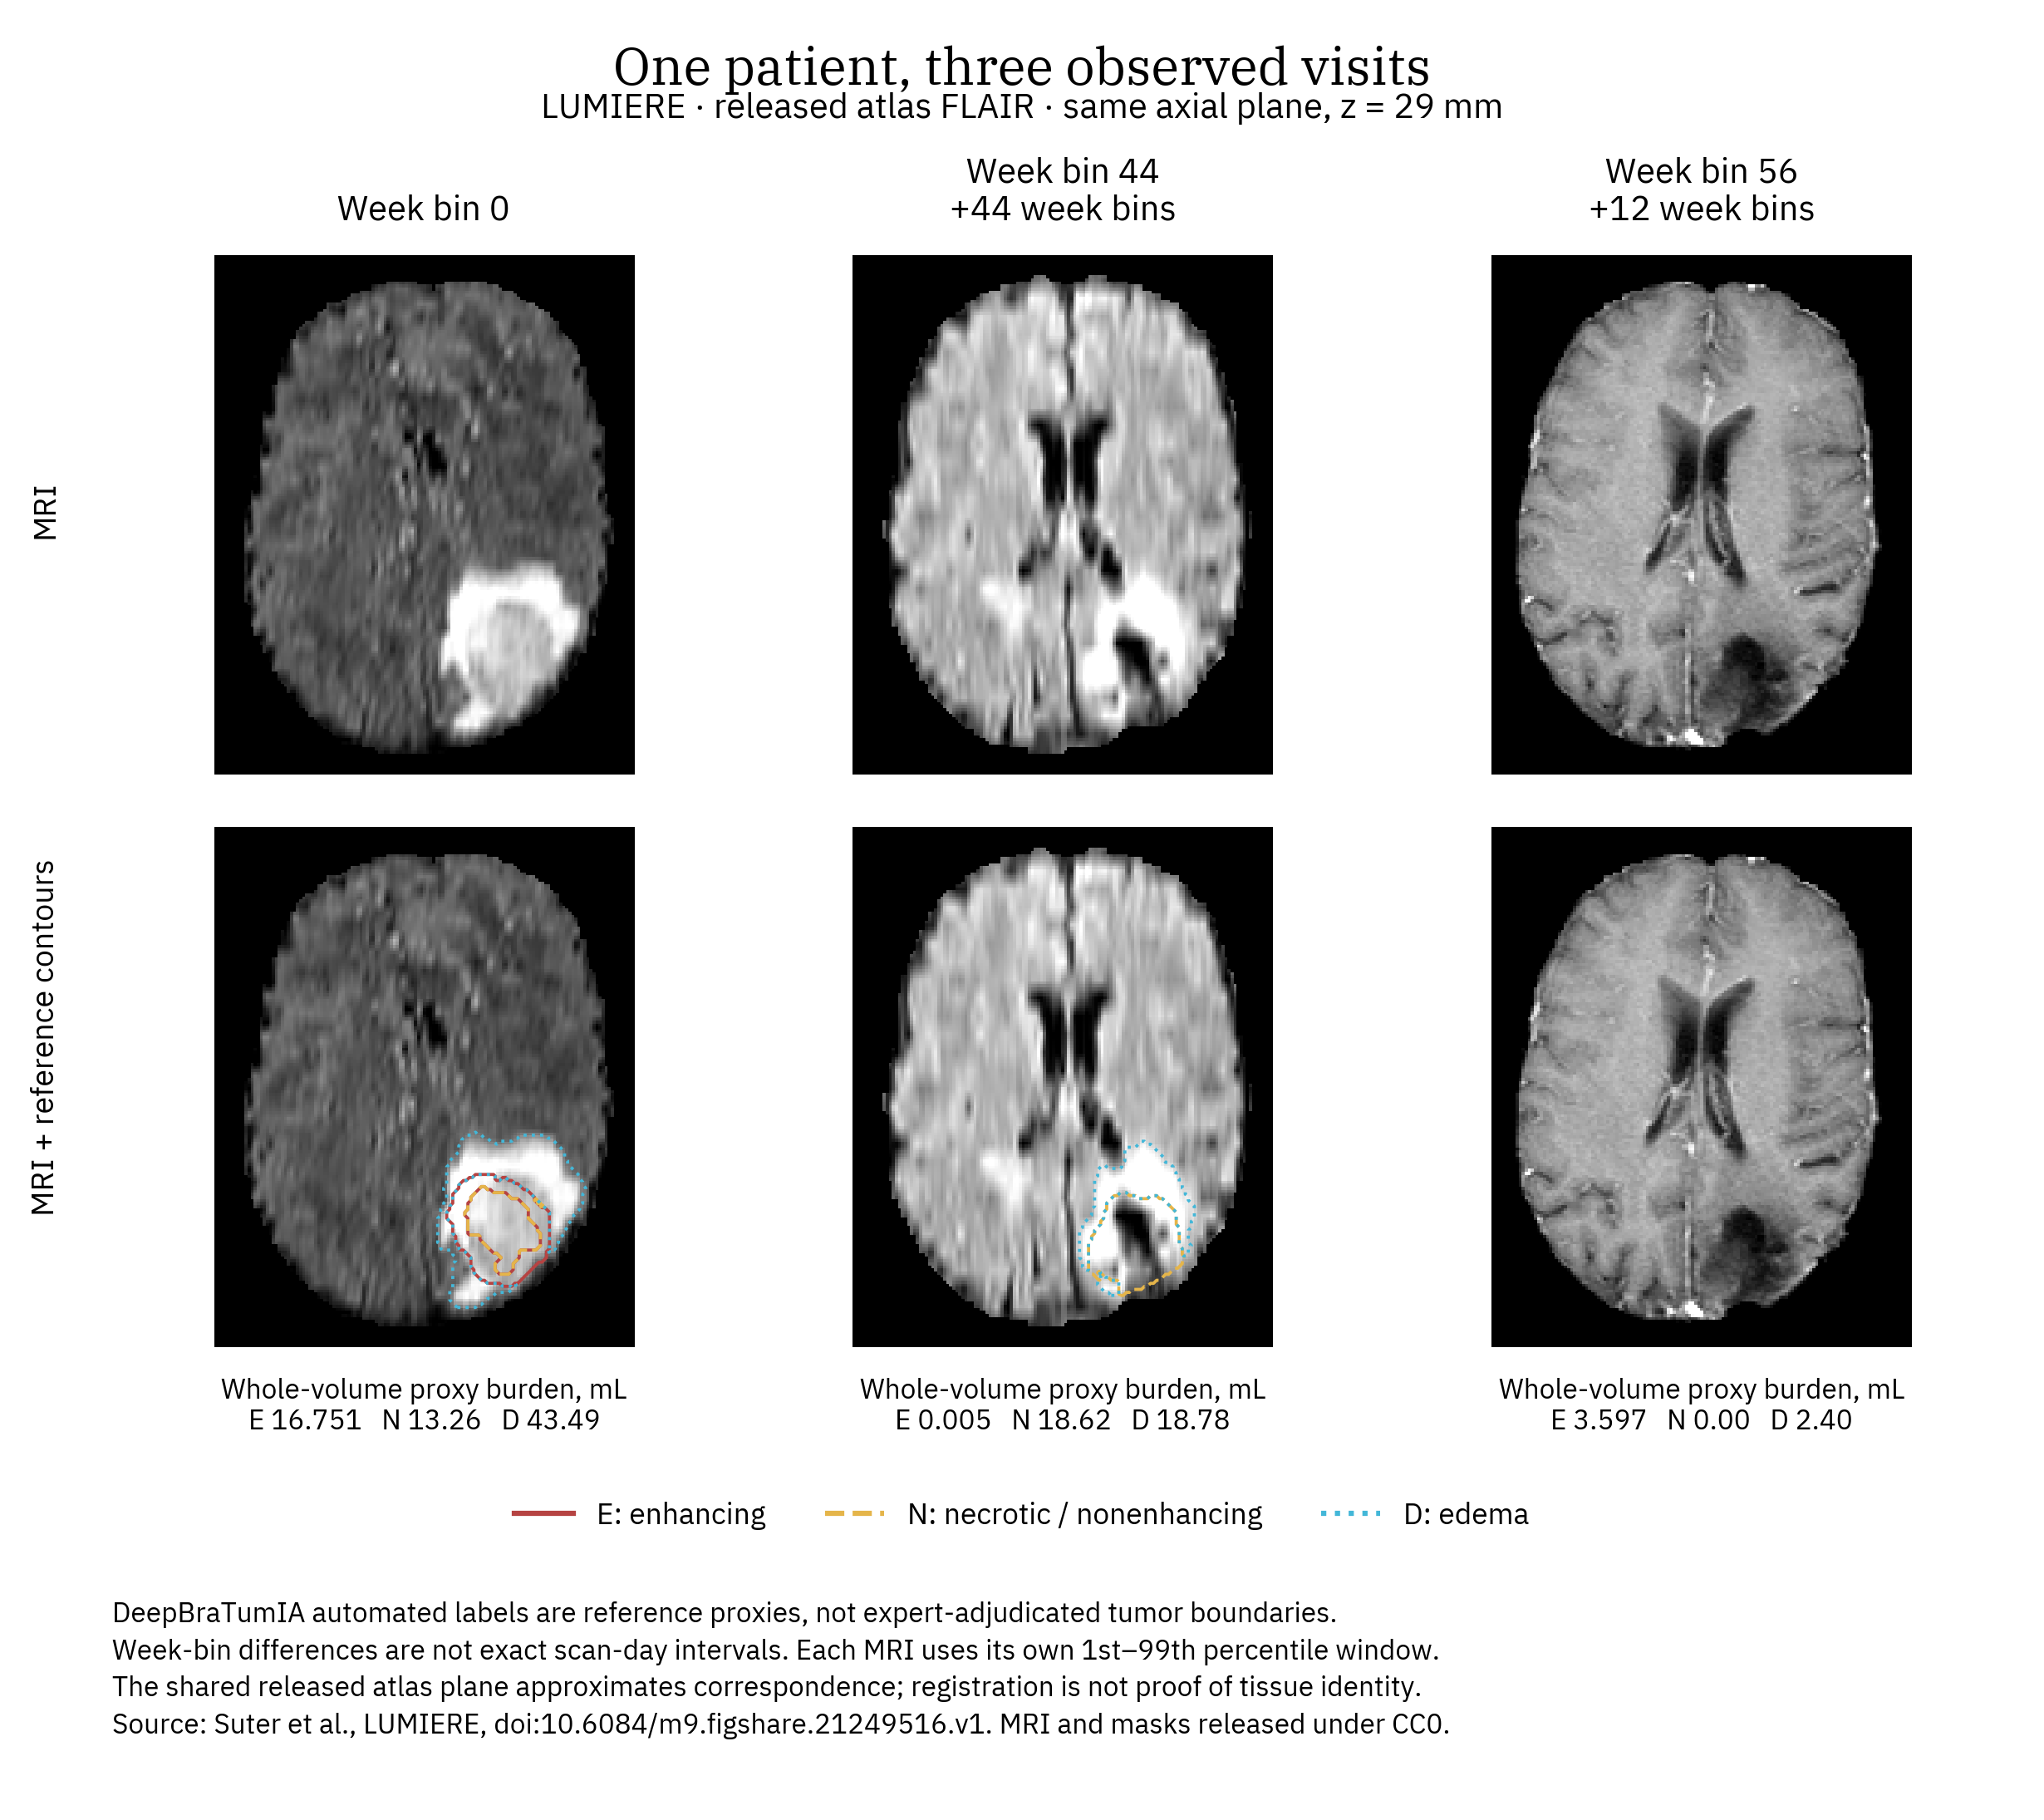
\includegraphics[width=\linewidth,height=0.55\textheight,keepaspectratio]{figures/figure_1_1.png}
\caption[Longitudinal FLAIR MRI and automated reference compartments]{FLAIR MRI and automated DeepBraTumIA compartments at week bins 0, 44 and 56, on the released atlas plane $z = 29$ mm. We selected the first patient in sorted order and the first complete visit in each of that patient's first three distinct week bins. The common slice maximizes summed reference foreground area across these visits. Week bins do not specify exact scan-day intervals, and the displayed visits need not be consecutive clinical examinations. Source: Suter et al., LUMIERE MRI and automated segmentations \cite{ref17}; CC0 1.0.}\label{fig:1.1}
\end{figure}

\clearpage
\chapter{Literature review}

Qazi et al. \cite{ref2} distinguish temporal prediction, action-conditioned prediction, counterfactual rollouts, and planning or control. MeWM, proposed by Yang et al. \cite{ref5}, combines a vision-language policy model with tumor-generative dynamics for treatment planning. Bai and Xiong \cite{ref14} learn directed temporal costs from trajectories to guide planning in a latent world model. Our study concerns temporal prediction from observed MRI visits. We need to establish what anatomy a learned state retains, how well it predicts later anatomy, and whether earlier visits improve that prediction.

\section{Learning features that retain anatomy}

I-JEPA, introduced by Assran et al. \cite{ref3}, predicts representations of target regions from context within the same image. Moving this idea to successive MRI visits changes the task: the target now belongs to a later observation, where the anatomy may have changed. A low error between feature vectors does not tell us how accurately the model predicted that change. We still need to recover anatomy from the features.

Medical adaptations of predictive learning account for anatomy and differences in image appearance. CheXWorld \cite{ref10} models local anatomical structures, their global arrangement and appearance-domain variation in radiographs. Neuro-JEPA \cite{ref11} uses a sparse latent predictive objective and a mixture-of-experts architecture to learn from T1-weighted, T2-weighted and FLAIR MRI.

Mager and Hansen \cite{ref12} combine predictive and contrastive objectives for structural MRI and evaluate retrieval, segmentation and age regression. Segmentation is particularly relevant to our study because it tests whether the features support recovery of spatial anatomy. Our same-visit mask and volume readouts serve that purpose. They let us assess current-state estimation before attributing forecast error to the temporal predictor.

\begin{samepage}
The evaluation cohort also matters. Li et al. \cite{ref13} pretrain a multimodal JEPA on computed tomography (CT) and linked clinical records for pulmonary nodule diagnosis. After supervised fine-tuning, their model achieved an internal area under the receiver operating characteristic curve (AUC) of 0.91, compared with 0.73 for imaging alone. On the external cohort, the corresponding AUCs were 0.72 and 0.75. The gain was specific to the internal evaluation. Transfer therefore needs to be tested separately when judging the value of a representation or an additional modality.

\end{samepage}

\section{Predicting later anatomy}

Predicting later anatomy also requires choosing how change enters the model. In TumorFlow, Biller et al. \cite{ref6} propagate spatial tumor-concentration fields with a biophysical growth model and condition MRI synthesis on those fields. This gives the predicted state a physical interpretation before an image is generated. In a learned feature space, we have to establish that interpretation through anatomical readouts.

Other approaches condition generation on observed scans and clinical inputs. Liu et al. \cite{ref7} use sequential imaging and treatment information to generate later MRI and tumor masks with a diffusion model. Huisman et al. \cite{ref9} use a rectified-flow model conditioned on pre-radiotherapy MRI, radiation-dose maps, timing and chemotherapy information. A dose map supplies the spatial distribution of radiation dose, which is more detailed than the recorded treatment-status variables available in our forecasting comparisons.

Laslo et al. \cite{ref8} make another conditioning choice explicit. Their guided diffusion model generates possible spatial growth in pediatric diffuse midline glioma from a baseline MRI slice and a target tumor area. In the longitudinal evaluation, the target area is known from the follow-up scan. The resulting comparison tests where growth occurs given its extent; it does not test whether the model can predict that extent from the baseline scan.

Table~\ref{tab:2.1} lists these inputs alongside the outputs being evaluated. Generated images allow direct inspection, but a plausible image can still contain the wrong anatomical change. For our forecasting question, both generated images and decoded feature predictions need to be compared with the patient's later anatomy. We then need to establish whether earlier visits helped.

\begin{table}[!htbp]\centering
\singlespacing\small\setlength{\tabcolsep}{4pt}\renewcommand{\arraystretch}{1.25}
\caption[Inputs and endpoints in selected prior work]{Inputs and endpoints in selected representation and prediction studies.}\label{tab:2.1}
\begin{tabular}{>{\raggedright\arraybackslash}p{\dimexpr 0.25\linewidth-2\tabcolsep\relax}>{\raggedright\arraybackslash}p{\dimexpr 0.38\linewidth-2\tabcolsep\relax}>{\raggedright\arraybackslash}p{\dimexpr 0.37\linewidth-2\tabcolsep\relax}}
\toprule \textbf{Study} & \textbf{Input or state} & \textbf{Prediction or evaluation} \\\midrule
Assran et al. \cite{ref3} & Observed image context & Representations of target image regions \\
Mager and Hansen \cite{ref12} & Structural MRI & Retrieval, segmentation and age regression from learned features \\
Biller et al. \cite{ref6} & Biophysical tumor-concentration fields & Conditioned MRI synthesis \\
Liu et al. \cite{ref7} & Sequential imaging and treatment information & Longitudinal MRI and tumor-mask generation \\
Huisman et al. \cite{ref9} & Pre-radiotherapy MRI, dose maps, timing and chemotherapy & Post-treatment MRI prediction \\
Laslo et al. \cite{ref8} & Baseline MRI slice and target tumor area & Spatial growth conditional on the supplied area \\
\bottomrule
\end{tabular}
\end{table}

\section{Timing and the contribution of history}

Clinical follow-up occurs at irregular intervals, and the date of the next scan may be unknown when a forecast is made. We therefore distinguish prediction at an unknown next-visit time from prediction at a supplied horizon, including cases where the realized interval is provided retrospectively.

Chen et al. \cite{ref15} compare five conditioning configurations with a shared architecture and training dataset in the cited first version of their retinal-imaging study. Aligning the input distributions used in training and inference improved image scores; differences among the aligned frameworks were not significant on the primary metrics. The study concerns retinal imaging, but illustrates how input conditioning can affect a comparison between forecasting methods.

For our study, the decisive comparison is between a model given MRI history and a matched model given only the latest MRI state, with the other inputs held fixed. Persistence establishes how well we can do by copying current anatomy. A latest-only model can improve on that baseline without using earlier scans, so beating persistence alone would not establish a benefit from history. With the current-state readouts, these comparisons let us judge anatomical recovery and the contribution of history separately.

\clearpage
\chapter{System specifications}

\section{Software requirements}

The software uses Python 3.11 or later. The uv environment manager, version 0.9.8 or later, installs dependencies at fixed versions.

PyTorch handles training and inference, MONAI for medical imaging operations, and NiBabel and SimpleITK handle image files and geometry. Pretrained-model adaptation uses PEFT with Transformers.

Experiments require local access to their cohort data. Pretrained models require official BrainIAC weights. Training ran on an RTX 5090 with 32 Gigabytes Of VRAM and 96 Gigabytes of system memory. The retained checkpoints, configurations and metrics document the completed runs.

\clearpage
\chapter{System design}\label{ch:design}
\begingroup
\clubpenalty=10000
\widowpenalty=10000
\brokenpenalty=10000

\section{Representing the patient state}

We use a patient state to connect MRI observations to anatomical predictions. The state needs to retain current anatomy in a form that a temporal model can use. We assess these requirements separately: anatomical readouts show what can be recovered from the state, while forecasting tests what it can predict about a later visit.

The compact JEPA branch encodes each visit as a feature vector and predicts the features of a later visit. Readouts convert those features into compartment volumes. The spatial branch retains feature maps and decodes masks as well as volumes, giving the decoder direct access to spatial information. Figure~\ref{fig:4.1} shows how the two representations connect observed MRI to future targets.

\begin{figure}[!htbp]\centering
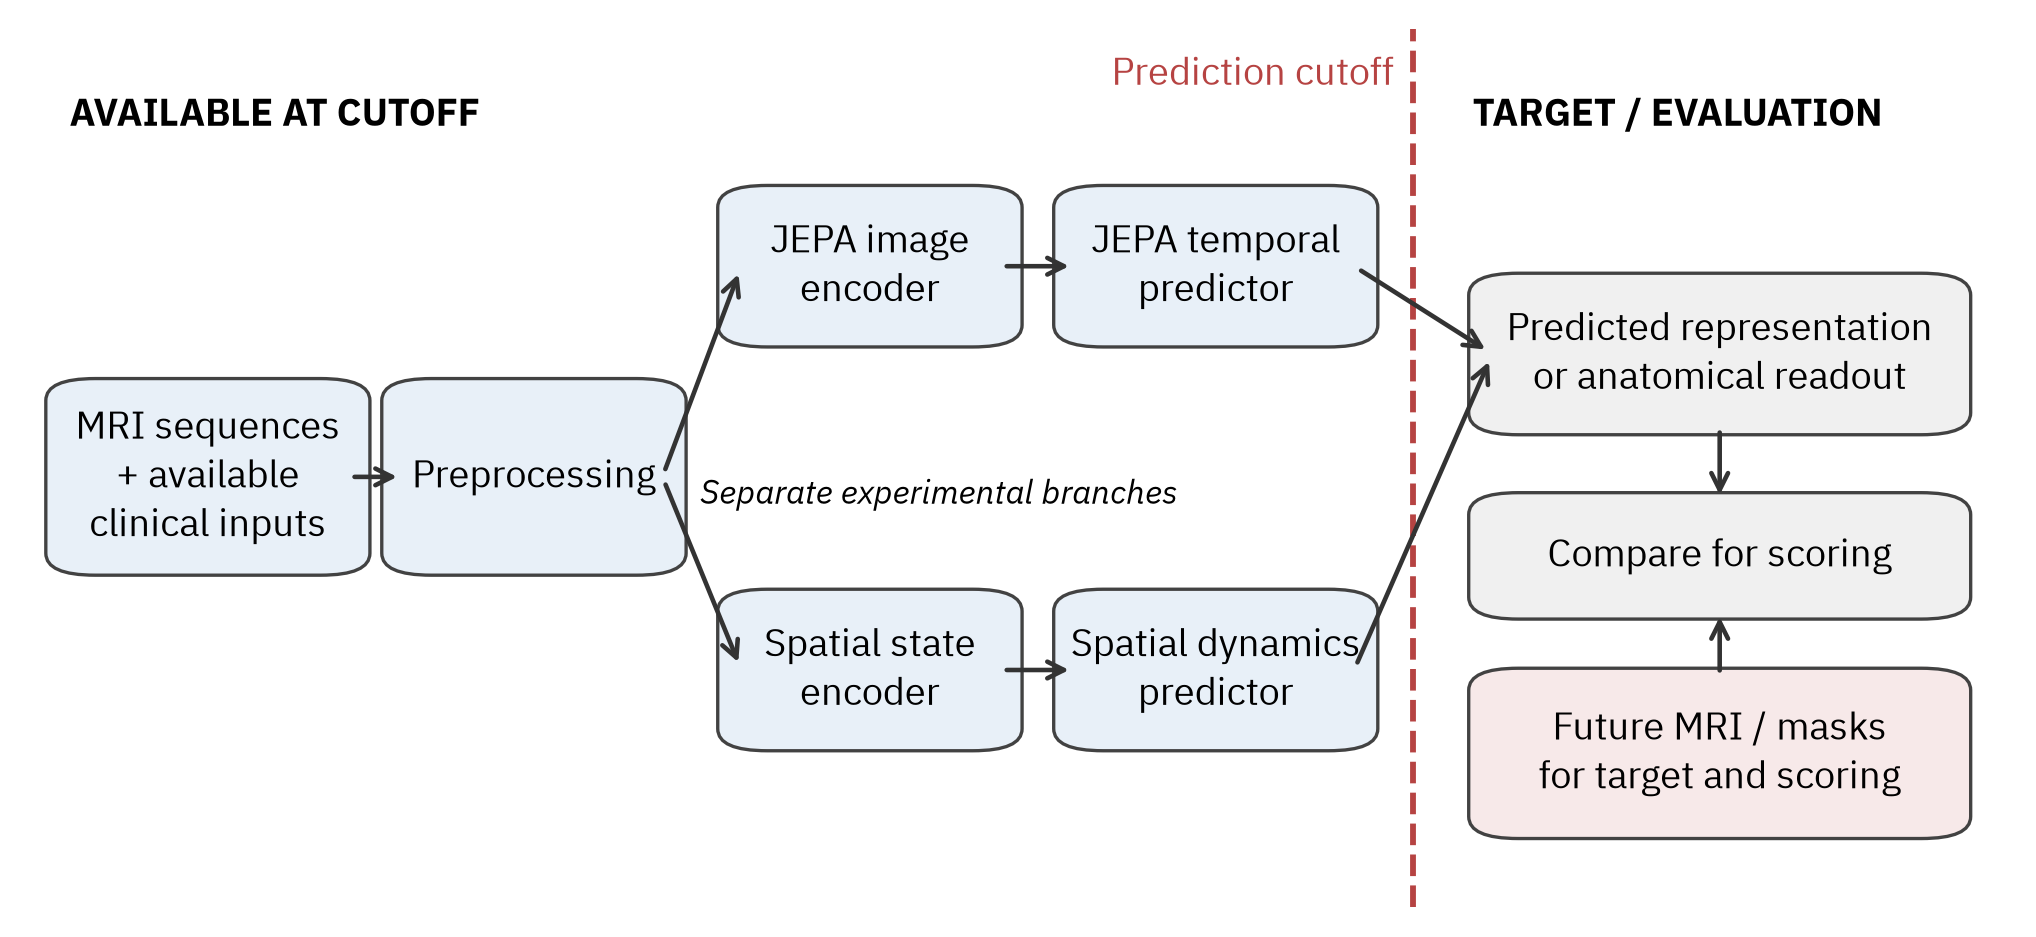
\includegraphics[width=\linewidth,height=0.57\textheight,keepaspectratio]{figures/figure_4_1.png}
\caption[Image-based experimental branches]{JEPA and spatial-state forecasting branches. Observed MRI forms the input; later MRI and masks provide targets for learning and evaluation.}\label{fig:4.1}
\end{figure}

\section{MRI inputs and anatomical supervision}\label{sec:cohorts}

The input sequences are T1, contrast-enhanced T1 (CT1), T2 and fluid-attenuated inversion recovery (FLAIR). Sequence-availability flags accompany the images so that the encoder can distinguish a missing sequence from an observed image with low intensity. Visits retain their order and past intervals when they enter a temporal model.

LUMIERE and SAILOR provide longitudinal MRI with automated anatomical references from DeepBraTumIA and ONCOHabitats respectively. Their compartments cover enhancing tumor, necrotic or nonenhancing tissue, and edema or FLAIR abnormality. MU-Glioma-Post provides neuroradiologist-reviewed masks with a separate resection-cavity label. These masks define the anatomical targets for the readouts.

Mask supervision gives the spatial encoder information about tissue location and boundaries. Volume supervision ties its features to anatomical burden. We measure physical volumes from the source segmentation and its voxel-to-world transform, before resizing masks for the network. For regional prediction, each labeled source voxel contributes its volume to one of eight fixed regions according to its center. This avoids losing small labeled structures through downsampling.

Cavity supervision gives the integrated observation model five output categories: background, enhancing tumor, nonenhancing core, FLAIR abnormality and cavity. LUMIERE has no cavity annotation, so its anatomical loss uses the four annotated categories. We evaluate both a conditional readout that removes the cavity logit and the native five-category readout. This makes the effect of the extra output category visible when comparing anatomical predictions.

\section{Learning from partial observations}

Missing-sequence completion gives us another way to test what the state retains. The model predicts withheld current FLAIR from the available sequences. Comparing CT1 alone with CT1 plus T1, and then with CT1 plus T1 and T2, tests the information added by each sequence. Giving the decoder higher-resolution spatial features tests whether it can use information that a compact state may lose.

A new readout fitted to a frozen state tests whether those features remain useful for another anatomical task. For segmentation, frozen random features and direct-image adaptation provide references for learned information and the cost of fixing the representation. The integrated observation model supports both anatomical decoding and missing-sequence completion from the same saved state.

History-assisted completion asks a related question about the present: whether a previous scan helps recover current FLAIR. Current images alone, genuine patient history and timing-matched donor history distinguish the contribution of the patient's own earlier observations. Registered previous-FLAIR persistence provides a reference for how much can be recovered simply by retaining the previous image.

\section{Forecasting from the observed state}\label{sec:cutoff}

A history model receives the current state and eligible earlier states, together with past timing. In the spatial branch, a recurrent predictor combines the feature maps and predicts a correction to the latest state. Its anatomical decoder maps the predicted features to future volumes. We also fit forecasts directly to measured volumes and previous measured change. This makes it possible to test the value of history without requiring an MRI encoder to recover those measurements first.

The main control is a matched latest-only model. It receives the current MRI state and the same timing and availability information, with earlier MRI features removed. For numerical volume models, the corresponding current-only control omits previous measured change. Matching the remaining inputs makes the comparison depend on the historical information being tested.

Persistence supplies a second reference by copying current anatomy to the target visit. Measured-volume persistence uses volumes from a current mask; decoded-state persistence uses the model's estimates from current MRI. The latter shares the state-estimation error of an MRI-based forecast. A latest-only predictor can improve on persistence, so the history comparison is needed to establish whether earlier visits add anything. Figure~\ref{fig:4.2} shows the information available on each side of the prediction cutoff.

\begin{figure}[!htbp]\centering
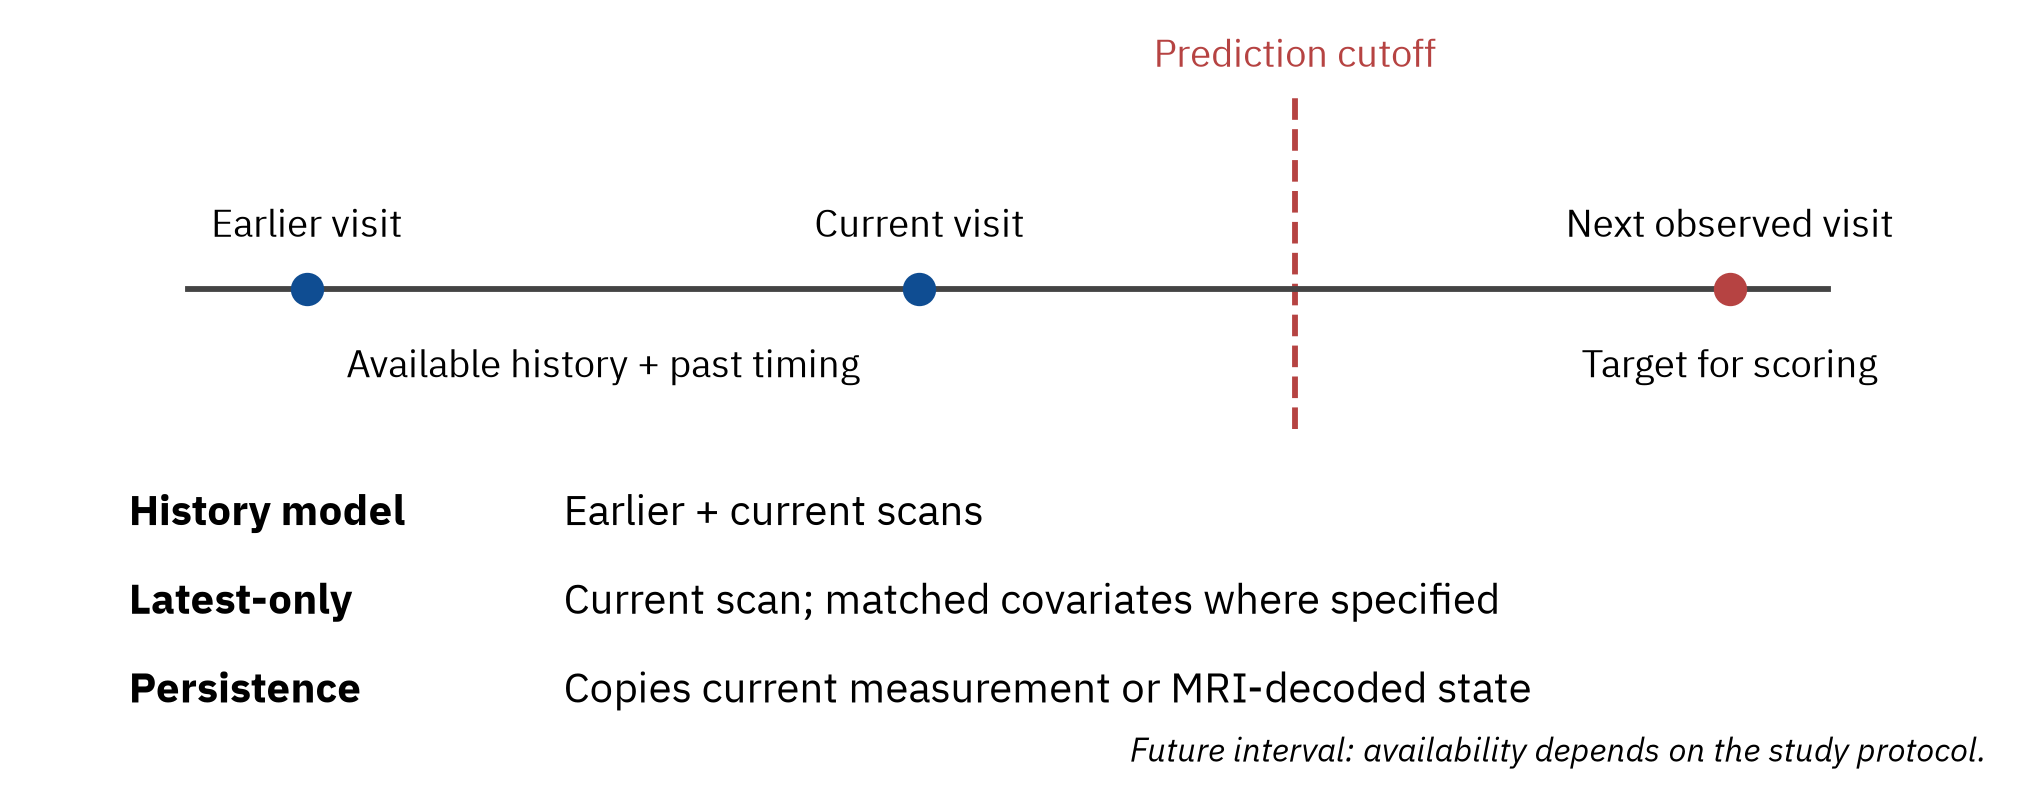
\includegraphics[width=\linewidth,height=0.57\textheight,keepaspectratio]{figures/figure_4_2.png}
\caption[Forecast inputs and comparison baselines]{History and latest-only predictors share the current observation. Persistence copies current anatomy, and the later observation supplies the target.}\label{fig:4.2}
\end{figure}

Next-visit models predict the next scan without knowing its interval in advance. Horizon-conditioned models receive an interval: the structured forecasts use requested horizons of 12 or 24 weeks, while retrospective comparisons supply the actual follow-up gap. LUMIERE intervals use nominal week bins; MU intervals use recorded days.

Completion can also prepare a representation for forecasting. We freeze the completion-adapted and original encoders and fit fresh matched history and latest-only heads to each. Both heads can use the latest observed FLAIR. This tests whether better recovery of a current image carries over to prediction of a later one.

Structured forecasts describe future anatomy through multiple anatomical scenarios. Compartment presence, amount and spatial allocation determine each scenario, with volumes computed from its segmentation. This keeps the predicted shape and burden consistent within a scenario. Quantity models isolate presence and amount before introducing spatial allocation: an accurate-looking boundary would be of limited use if the model predicted the wrong amount of tissue. Scalar-volume controls test whether MRI features add predictive information beyond current anatomical measurements. Recorded treatment status can also enter as an additional covariate in a matched forecast comparison.

\section{Choosing another MRI sequence}

The state also supports a choice about what to observe next. Starting with T1, the acquisition model chooses which available sequence to reveal. The JEPA selector uses predicted features of a candidate sequence alongside the observed state; the direct selector uses the observed state alone. Once the chosen MRI is revealed, it updates the state.

We compare both selectors with a fixed acquisition order at budgets of two and three observed sequences. Their utility is the anatomical score at those budgets, so a useful choice must improve the state available for anatomical prediction. An oracle that chooses using target outcomes estimates how much improvement is available under the same observer. This separates the quality of the selection rule from the observer's ability to benefit from an additional sequence.

\section{Evaluation design}\label{sec:evaluation}

The comparisons follow the role of each component. Current-state tests assess anatomical recovery, forecast tests assess later anatomy, and acquisition tests assess the value of another observation. Table~\ref{tab:4.1} summarizes the main questions and the controls that make them interpretable.

\begin{table}[!htbp]\centering
\singlespacing\small\setlength{\tabcolsep}{4pt}\renewcommand{\arraystretch}{1.2}
\caption[Design questions and matched comparisons]{Design questions, matched comparisons and anatomical endpoints.}\label{tab:4.1}
\begin{tabular}{>{\raggedright\arraybackslash}p{\dimexpr 0.25\linewidth-2\tabcolsep\relax}>{\raggedright\arraybackslash}p{\dimexpr 0.46\linewidth-2\tabcolsep\relax}>{\raggedright\arraybackslash}p{\dimexpr 0.29\linewidth-2\tabcolsep\relax}}
\toprule \textbf{Question} & \textbf{Comparison} & \textbf{Endpoint} \\\midrule
Does initialization help? & Pretrained and random encoders with matched architecture and supervision & Current masks and volumes \\
Does spatial access help? & Higher-resolution decoder features enabled or zeroed & Current FLAIR and local image detail \\
Does history help forecasting? & History versus latest-only or current-only, with persistence as a reference & Future anatomy and volume distributions \\
Does history help completion? & Current images alone, genuine history and donor history & Withheld current FLAIR \\
Does sequence selection help? & JEPA selector, direct selector and fixed order & Anatomy after two and three sequences \\
\bottomrule
\end{tabular}
\end{table}

Mean absolute error (MAE) scores a point prediction, while the continuous ranked probability score (CRPS) scores a predictive distribution. Lower is better for both. Dice measures segmentation overlap from zero to one. Empty and nonempty reference compartments are reported separately where required, since predicting absence and recovering the shape of present tissue are different tasks.

The volume endpoint depends on the model. Whole-compartment regression comparisons use log1p(mm³), the logarithm of one plus numerical volume in cubic millimetres. Corrected regional forecasts use log1p(mL), and structured and quantity forecasts score volumes in mL. Image errors use standardized intensity. We compare models on the same target and scale, rather than ranking absolute errors across these endpoints.

For scenario forecasts, Dice scores the weighted vote of the segmentations and volume MAE scores the distribution mean. A displayed scenario is one possible output. The final quantity comparisons compute core mean-volume and CRPS scores from the fitted discrete distribution, avoiding dependence on a small scenario sample.

Patients contribute different numbers of visits, so we average eligible observations within each patient before averaging across patients. Multi-seed results average scores from separately fitted models; repeated-partition comparisons average their partition scores. Paired bootstrap intervals resample patients while keeping competing predictions together. We judge a gain through its size and uncertainty, alongside consistency across patients and fitted models. The task-specific scoring definitions and decision criteria are given in the methods \cite{record}, with paired results in Chapter~\ref{ch:results}.

\endgroup

\clearpage
\chapter{System implementation}\label{ch:implementation}
\begingroup
\clubpenalty=10000
\widowpenalty=10000
\brokenpenalty=10000

The implementation follows the patient state from MRI inputs to anatomical and image outputs. Encoders build a compact visit vector, a spatial feature grid, or a hierarchy of feature maps. We keep readouts and temporal predictors separate from these encoders so that each can be tested while the others remain fixed.

\section{Preparing images and longitudinal batches}

The BrainIAC input pipeline applies N4 bias-field correction, isotropic resampling and brain extraction before preparing a 96 × 96 × 96 array. Rigid registration uses an MNI template when one is supplied. Nonzero intensity normalization computes the mean and standard deviation over the image foreground, keeping background voxels out of those statistics. We retain the pre-resize geometry for physical measurements: anatomical volumes come from source masks, while the resized arrays provide network inputs.

The longitudinal batch arranges MRI by patient, visit and sequence. Padding gives patients with different numbers of visits a common tensor shape. A visit mask identifies real visits, and a sequence-availability mask identifies loaded images. The image encoder processes the available sequences, and a JEPA prediction pair requires MRI at both its observed and target visits. Clinical features are encoded separately before fusion; treatment-status regressions use the status recorded at the cutoff session as an input distinct from response-assessment labels.

\section{JEPA encoding and temporal prediction}

The compact image encoder is a three-dimensional Vision Transformer initialized from BrainIAC weights \cite{ref16}. Each sequence produces a 768-component vector. We average the available sequence vectors to form a visit representation, so its size stays fixed when a sequence is missing. Low-rank adaptation updates small parameter matrices in selected linear layers while the base weights remain frozen.

For multimodal prediction, we normalize the clinical and image features and concatenate them into a visit token. We add timing encodings before passing the tokens to the temporal Transformer. At a given cutoff, the Transformer receives only the prefix ending at that visit. The output at the last real visit becomes the temporal state; the visit mask keeps padding out of the attention calculation.

A multilayer perceptron maps this temporal state into the target feature space. The target encoder is a copy of the image backbone and projection head, updated through an exponential moving average of their parameters. It runs in evaluation mode without gradients, providing a slowly changing target as the online encoder learns. The prediction loss is one minus the cosine similarity between normalized predicted and target features.

Figure~\ref{fig:5.1} shows how the two paths meet at the loss. Anatomical readouts then map the learned representations to compartment volumes, making the forecast interpretable in the same units as the anatomical targets.

\begin{figure}[!htbp]\centering
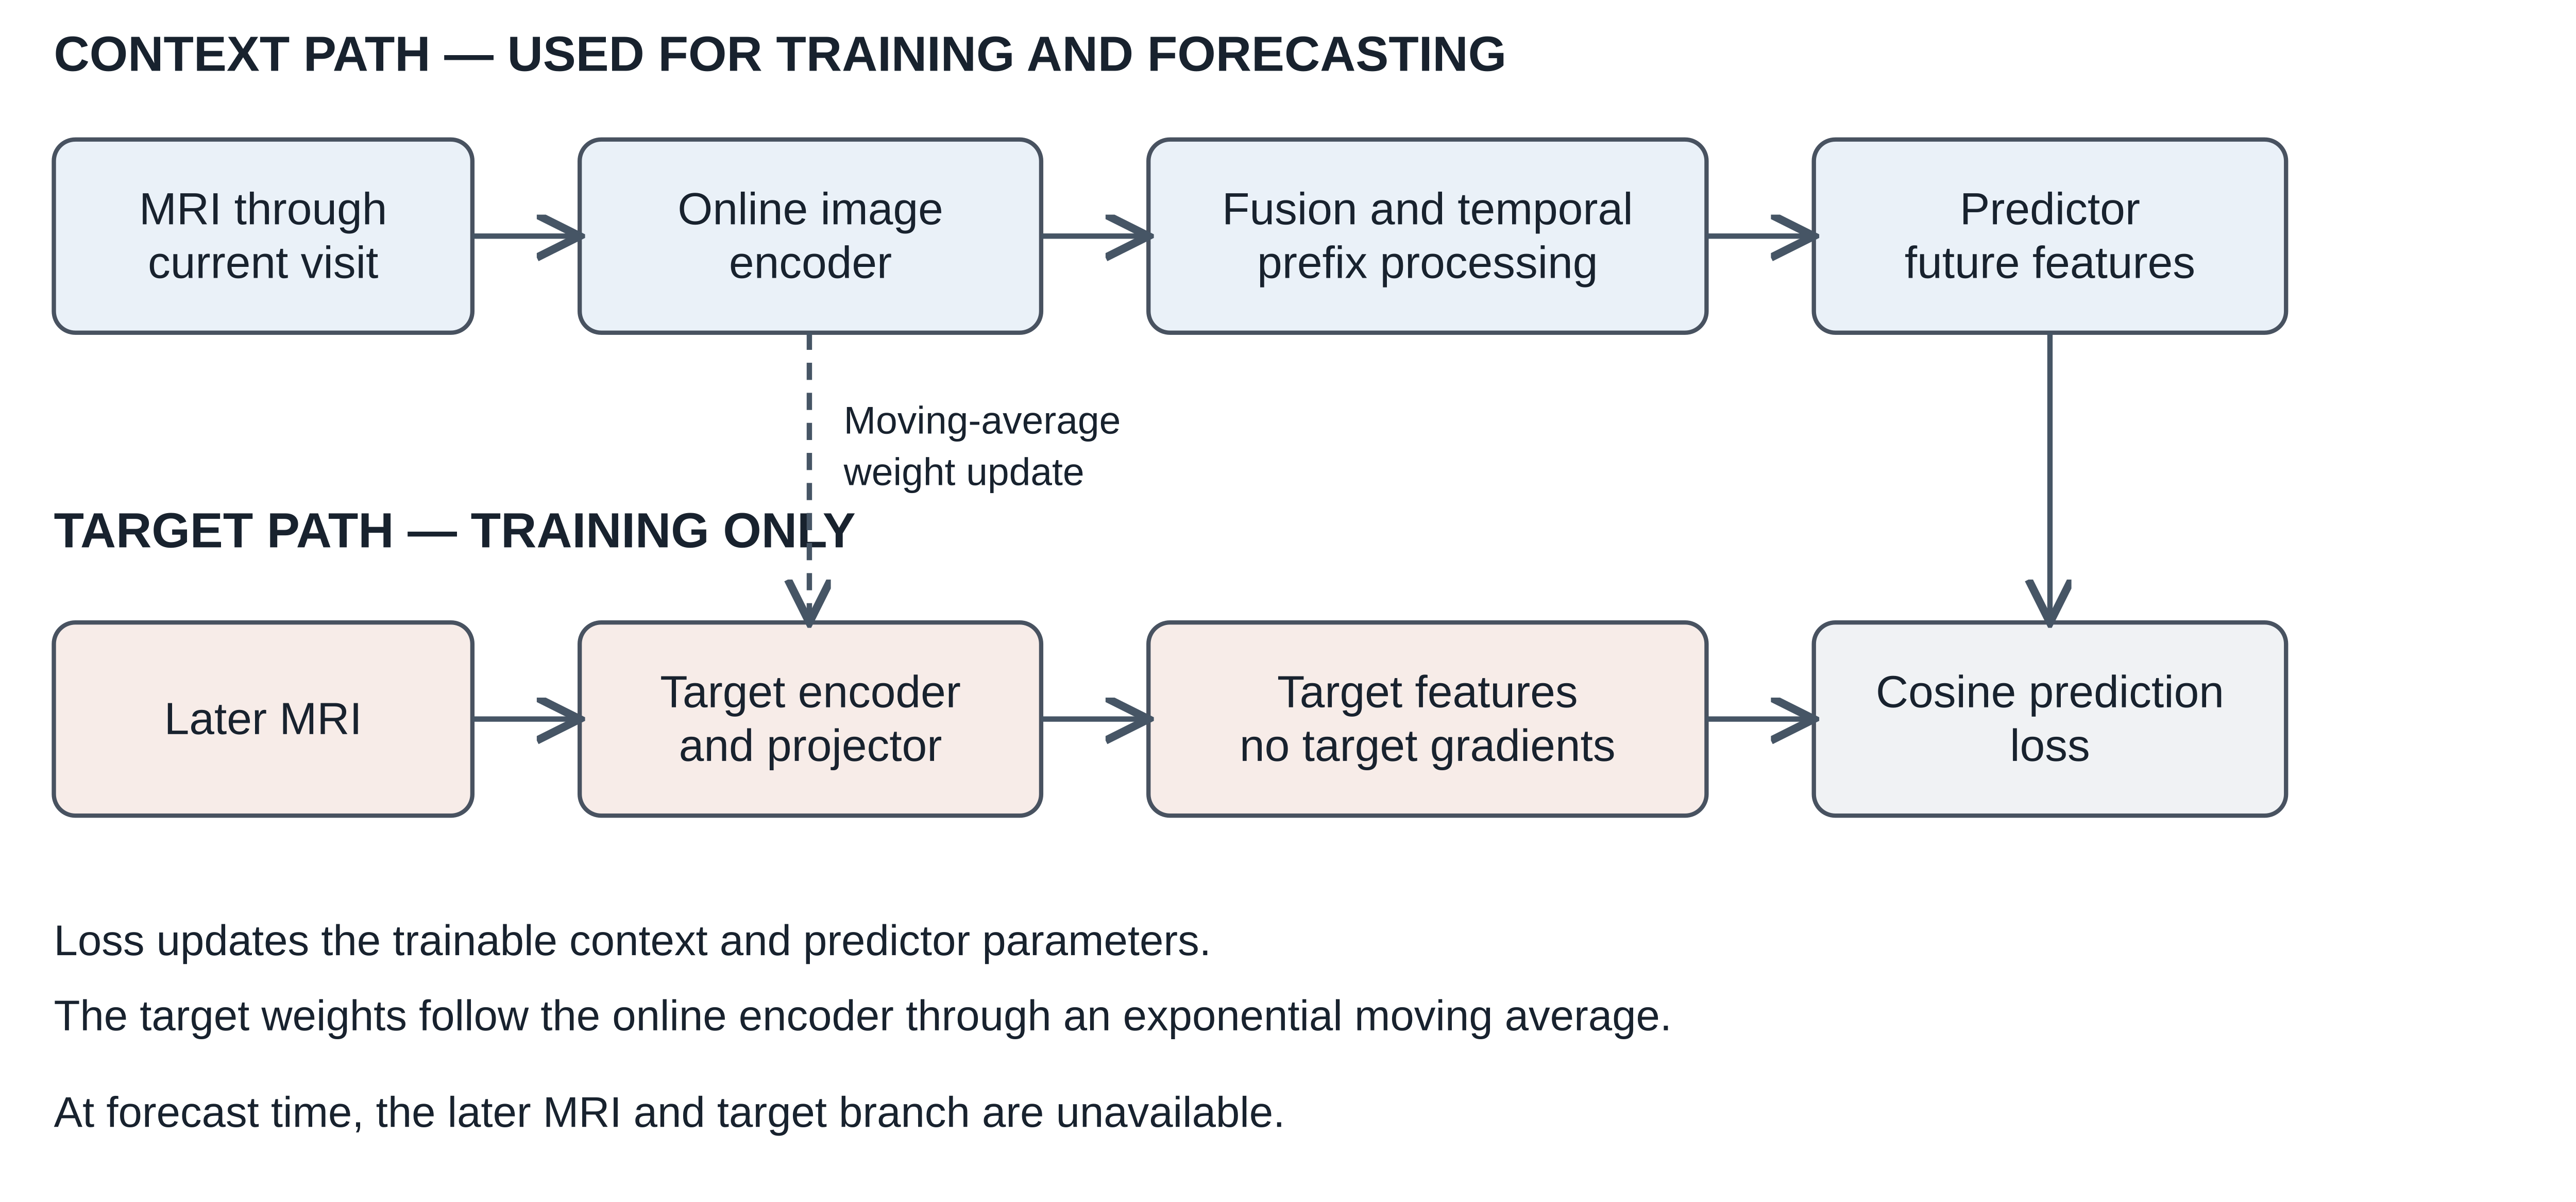
\includegraphics[width=\linewidth,height=0.57\textheight,keepaspectratio]{figures/figure_5_1.png}
\caption[JEPA training paths and the context path retained for forecasting]{JEPA context and target paths. The target encoder and projector follow their online counterparts through a moving-average update.}\label{fig:5.1}
\end{figure}

\section{Spatial states and anatomical readouts}

The convolutional spatial encoder receives four MRI channels and four sequence-availability channels. Its residual three-dimensional blocks have widths of 16, 32, 64 and 128. A decoder combines their spatial maps to predict three compartment masks, while spatially averaged features feed a three-output volume head. Binary cross-entropy and Dice loss train the masks; absolute error on standardized log-volume targets trains the volume readout. For observed-change prediction, a paired model processes two available scans. The independent-state control instead subtracts their separately estimated volumes.

The spatial-token encoder keeps a different form of state. It retains the Vision Transformer's sequence-specific tokens on a 6 × 6 × 6 grid, fuses them into 64 channels, and decodes masks at 24 × 24 × 24. This preserves spatial inputs to the readout instead of reducing each visit to one vector. Pretrained and random versions share the architecture, supervision, training draws and initial non-backbone weights, with all encoder parameters trainable. Their comparison therefore changes initialization while keeping the decoding problem fixed.

The integrated observation model retains higher-resolution encoder maps alongside the compact state. Both its anatomical decoder and its missing-sequence decoder read these saved features. Cavity supervision covers the full annotated field, including labeled cavity outside the MRI foreground, while image losses use the MRI foreground. Keeping those supports separate allows the anatomical loss to include all annotated tissue without filling the image objective with background voxels.

\section{Completing and predicting FLAIR}

The token-based completion model predicts current FLAIR from CT1, T1 and T2. BrainIAC supplies all 216 spatial tokens for each sequence. A fresh head projects their concatenated features to 64 channels and upsamples the 6 × 6 × 6 grid through convolutional blocks to 96 × 96 × 96. We fit the same head with either an adapted encoder or the original frozen encoder to test what completion training adds to the representation.

For future-image prediction, each encoder is frozen and receives fresh matched forecast heads. A recurrent unit combines non-FLAIR tokens across visits at each spatial location. The decoder predicts an image residual that is added to the latest observed FLAIR. This gives the model a direct persistence path and leaves it to learn the correction. History and latest-only heads share that path and the same past timing; earlier FLAIR is excluded from the history representation. Completion and forecasting both minimize image MAE in a fixed field derived from fitting-patient T1 images.

\section{Predicting change in spatial features}

The frozen-state predictor holds the anatomical encoder and volume head fixed while learning how their state changes. It reduces 128-channel maps to a 16-channel recurrent state and processes up to four visits with a convolutional gated recurrent unit. Past gaps and sequence-availability flags enter alongside each map. A residual head predicts a correction to the latest map, and a scale head produces 128 positive uncertainty scales.

The frozen affine volume decoder converts the predicted feature means and scales into Gaussian log-volume distributions. Training minimizes anatomical CRPS plus 0.1 times standardized feature-mean squared error. The anatomical term connects the prediction to the quantity being evaluated, while the feature term keeps the predicted state tied to the encoder's representation.

We implement the history controls by changing the earlier maps at the predictor input. Latest-only replaces them with zeros but retains their timing, availability flags and visit mask. Pooled history replaces each earlier map by its spatial mean. These changes distinguish the contribution of earlier images from the contribution of their spatial detail.

Gradient routing determines whether the state itself can adapt to forecasting. Joint training lets forecast losses update the encoder. Observation-only training detaches the encoder from forecast losses while continuing to train its current-anatomy readouts. The supplied-horizon variant adds the realized week-bin interval to both history and latest-only predictors and compares spatial recurrence at two resolutions.

\section{Forecasting from anatomical measurements}

Ridge regression provides a forecast directly from anatomical quantities. Treatment-status models use saved volume estimates from the spatial encoder, adding the preceding state difference for history and current treatment status with its state interactions. Inner patient folds select the ridge penalty and estimate residual uncertainty; outer folds provide predictions for patients outside that fit. Measured-state models use whole-compartment reference volumes, with horizon-aware variants adding the supplied interval and interactions with current volume and prior velocity.

Regional models use source-mask measurements. Each labeled voxel contributes its physical volume to the region containing its center. The implementation records out-of-field volume separately so that regional and outside totals can be checked against the source total. Eight regions give 24 region-compartment values for LUMIERE and 32 for MU-Glioma-Post, which includes cavity.

The numerical predictors comprise persistence, mean change, constrained trend extrapolation, current-only ridge, history ridge and shuffled history. Current-only ridge uses current measurements and the past gap; history adds the previous measured change. We standardize features using fitting patients, giving each patient equal total weight. The ridge penalty is selected from 0.01, 0.1, 1, 10 and 100 by minimum selection MAE. Predictions are clipped at zero because volumes cannot be negative. Each cohort has its own fitted coefficients and normalizers.

\section{Structured anatomy and quantity models}

The structured forecaster represents possible futures as anatomical scenarios. It conditions spatial changes on current images, predicted anatomy and, in the history version, the previous observed change. Current volumes, timing and the requested horizon determine scenario coefficients and mixture weights. Each scenario supplies a segmentation and the volumes measured from it, keeping its shape and burden consistent. Scalar controls predict volume distributions from the corresponding current or historical quantities.

The quantity model separates compartment presence and amount from spatial allocation. It fits presence and voxel counts, constraining each count by the remaining available voxels and reserving space for later compartments sampled as present. Exact discrete cumulative distributions provide deterministic core mean-volume and CRPS scores. This lets us assess the fitted quantity distribution directly, without making its score depend on a small sample of anatomical scenarios.

\section{Selecting another MRI sequence}

The acquisition model uses a shared sequence encoder and order-independent fusion: the same observed sequences produce the same state regardless of reveal order. A hypothetical-feature predictor estimates the representation of a candidate sequence. Matched ridge selectors use features of the observed state, with the JEPA selector receiving an additional block of predicted candidate features and the direct selector using zeros in that block.

When a sequence is revealed, its actual MRI updates the observed state. The anatomical and completion decoders then read the updated features. Hypothetical features guide the choice of sequence, while the saved observation state contains the features of images actually received. This keeps the acquisition decision connected to the same readouts used to assess the representation.

\section{Training and restoring the models}

The JEPA trainer uses AdamW with learning-rate warmup and cosine decay. Mixed precision, chunked image encoding and activation checkpointing reduce memory use. Gradient accumulation combines several small batches into one optimizer update. In pair-weighted accumulation, each batch contributes according to its valid prediction-pair count. The learning-rate schedule and moving-average target update advance with optimizer steps, so their rate of change follows parameter updates rather than individual batches.

Checkpoint selection follows the output being learned: anatomical CRPS for probabilistic forecasting, nonempty-compartment Dice for the matched anatomical encoder, and image MAE for completion and image prediction. The frozen-state forecast also selects an uncertainty multiplier on selection patients. Ties retain the earlier checkpoint, and numerical regressions choose their penalties before final scoring.

Saved checkpoints contain model parameters, optimizer state, epoch and configuration. Evaluation restores the fitted normalizers and readouts with the weights because all three determine the prediction. Stored features retain patient, visit and encoder identities so that competing predictors can use the same observations. Chapter~\ref{ch:testing} describes the checks that saving, restoring and scoring these components reproduce their outputs.

\endgroup

\clearpage
\chapter{System testing}\label{ch:testing}
\begingroup
\clubpenalty=10000
\makeatletter\@clubpenalty=10000\makeatother
\widowpenalty=10000
\brokenpenalty=10000

The main comparisons depend on recovering anatomy from the right observations and measuring its change consistently. We therefore test the path from source masks and MRI inputs through model updates to the reported scores. Synthetic cases provide known answers, short real-data checks exercise the training path, and saved predictions allow independent scoring. Together, these checks support the distinction between recovering current anatomy and predicting future anatomy that runs through the report.

\section{Preserving geometry and physical volume}

Geometry tests cover axis flips, translations, anisotropic voxels and mismatched MRI-sequence grids. The loader checks finite image values and valid mask labels before measurement. Masks are aligned using their source and MRI transforms: resizing them independently as arrays can place otherwise valid labels in the wrong anatomical location.

Correct alignment alone does not preserve volume. Coarse nearest-neighbor sampling can discard a small labeled region even when the source mask contains positive volume. Across 322 inspected visits, coarse counting erased 605 of 7,728 regional compartment measurements. Among 5,784 regional changes, 102 reversed direction relative to source-volume aggregation. Figure~\ref{fig:6.1} shows these discrepancies across the fitting, selection and scoring partitions. A forecast trained on those targets could learn the effect of sampling rather than anatomical change.

\begin{figure}[!htbp]\centering
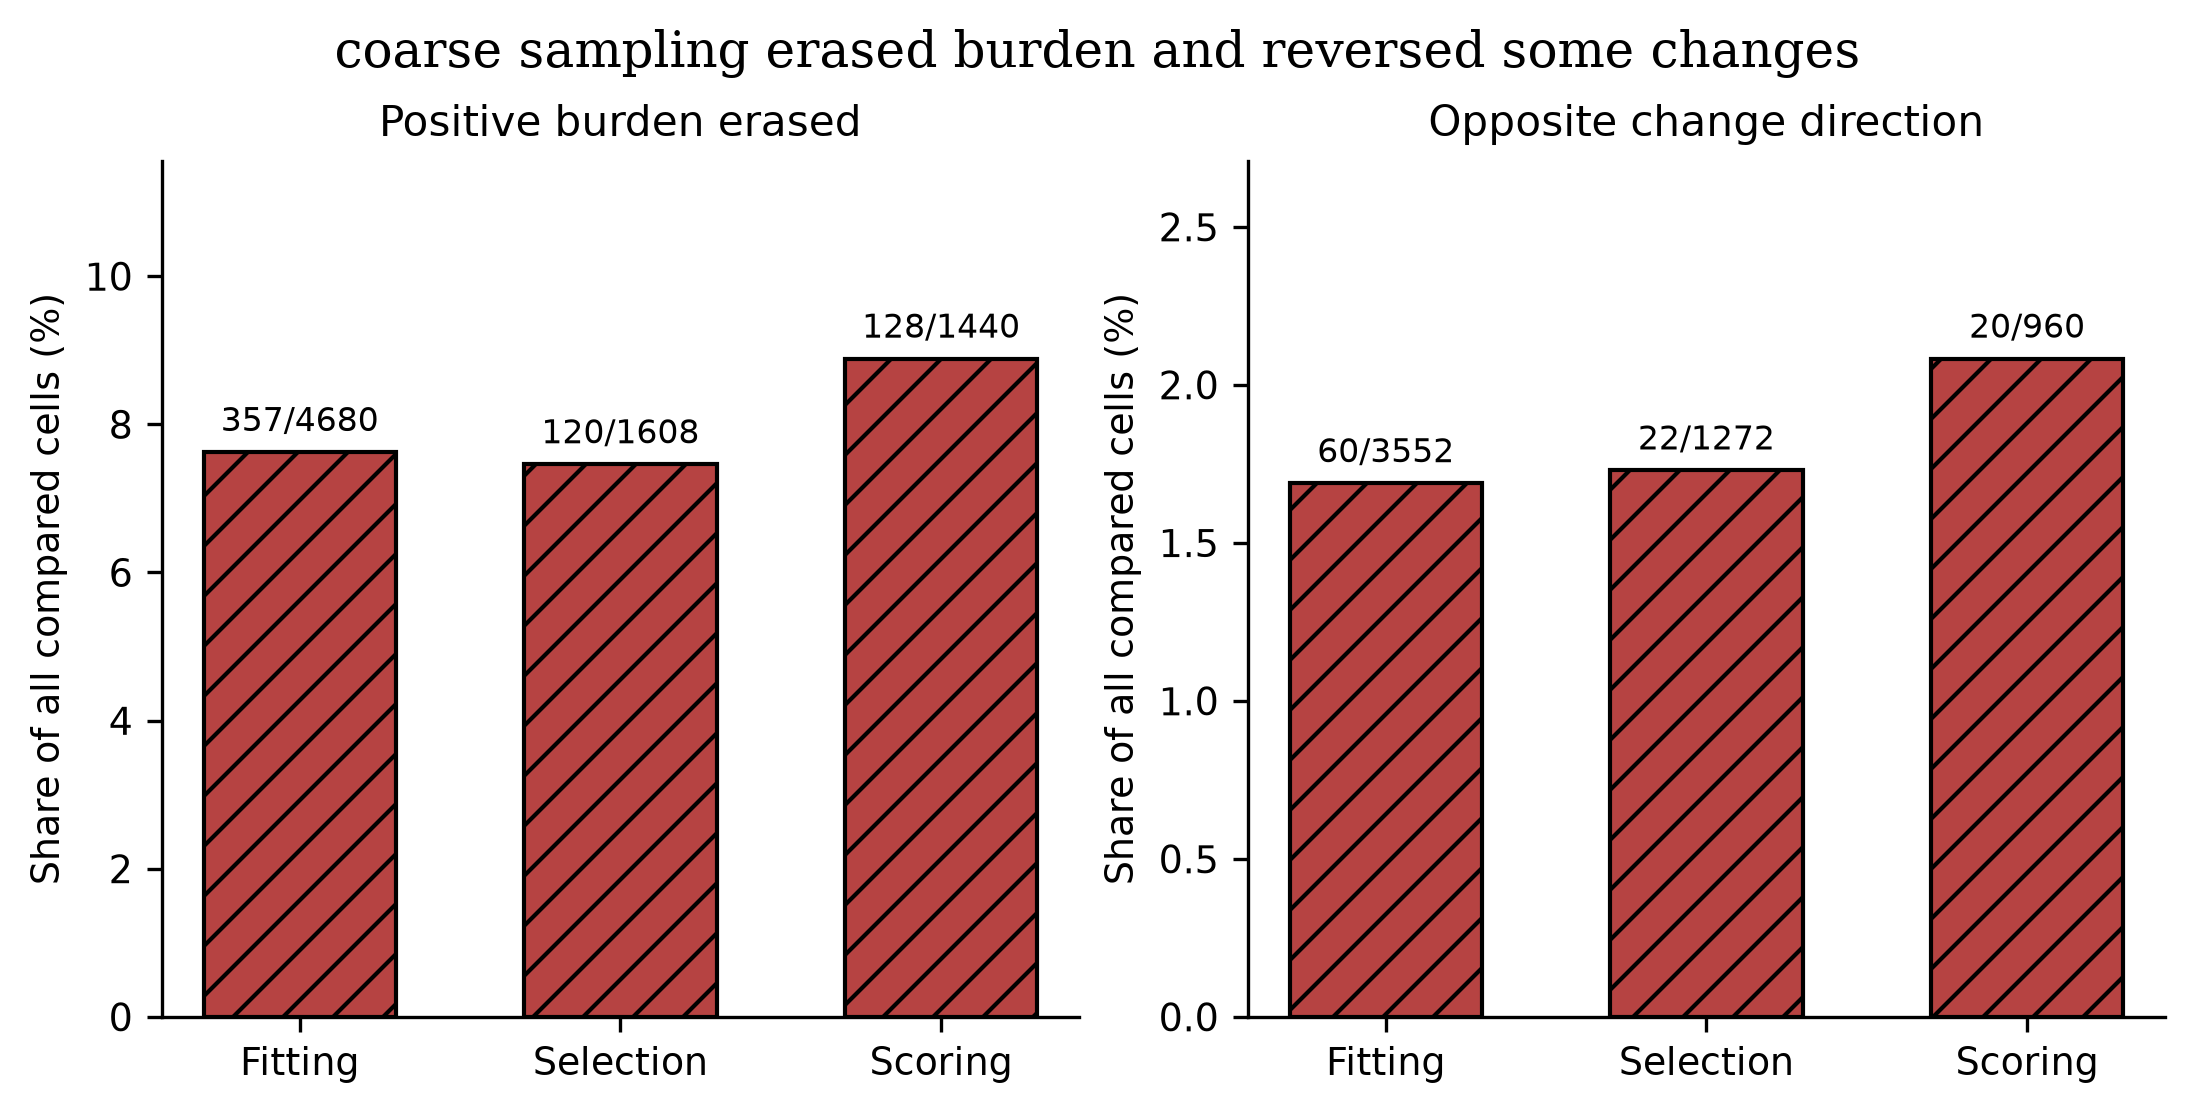
\includegraphics[width=\linewidth,height=0.57\textheight,keepaspectratio]{figures/figure_6_1.png}
\caption[Information lost through coarse mask sampling]{Regional target discrepancies across 322 visits. Each bar divides the number of affected region-compartment measurements or changes by all corresponding comparisons in that partition. Counts are printed beside the bars. These pooled counts describe the inspected cohort, with no sampling interval.}\label{fig:6.1}
\end{figure}

We measure regional volume by assigning each source voxel's physical volume to its region. Tests require regional and out-of-field totals to conserve the source total, preserve exact zeros for empty masks, and reject invalid labels. Independent extraction reproduced the regional volumes for all 322 visits. The targets retain physical units and visit order, and the regional regressions use newly fitted normalizers for these measurements.

\section{Enforcing the prediction cutoff}

Chronology checks preserve LUMIERE visit order using week bins and within-week suffixes. Forecast pairs refer to the original visit sequence, so removing an unusable intermediate scan cannot silently redefine the next visit. MU pairs require complete, increasing scan times.

A predictor must also be insensitive to information excluded by its cutoff. The tests replace future fields and verify that forecast inputs and predictions remain unchanged. Changing held-out outcomes must leave fitted parameters and predictions unchanged as well. These assertions address failure modes found during development: an earlier forecasting path admitted later-visit images, masks and interval features, and a clinical loader included eventual survival. The affected forecasting gains were withdrawn, and survival is excluded from default clinical inputs. Table~\ref{tab:6.1} summarizes the input and component checks.

\begingroup\singlespacing\small\setlength{\tabcolsep}{4pt}\renewcommand{\arraystretch}{1.25}
\begin{longtable}{>{\raggedright\arraybackslash}p{\dimexpr 0.5\linewidth-2\tabcolsep\relax}>{\raggedright\arraybackslash}p{\dimexpr 0.5\linewidth-2\tabcolsep\relax}}
\caption[Component and information-cutoff checks]{Assertions used to test model behavior and the information available at prediction time.}\label{tab:6.1}\\
\toprule \textbf{Test case} & \textbf{Expected behavior} \\\midrule\endfirsthead
\toprule \textbf{Test case} & \textbf{Expected behavior} \\\midrule\endhead
\bottomrule\endfoot
Padding and availability & Adding masked padding leaves the prediction unchanged; malformed availability flags are rejected. \\
Forward and backward pass & Outputs, losses and gradients remain finite; the intended trainable parameters receive gradients. \\
Frozen components & Frozen decoder or encoder parameters remain unchanged while gradients can reach the trainable predictor. \\
Checkpoint round trip & Saving and restoring the model reproduces its predictions and optimizer state. \\
Known metric fixture & CRPS agrees with a known analytic case; patient weighting matches an explicitly calculated result. \\
Future-input perturbation & Changing excluded future fields cannot alter the constructed forecast inputs or prediction. \\
Held-out-target perturbation & Changing held-out outcomes does not alter a fitted prediction or fitted model parameters. \\
\end{longtable}\endgroup

\section{Exercising training and saved states}

Short real-data checks exercise the complete training path: loading one or two batches, computing forward and backward passes, updating weights, and saving and restoring a checkpoint. They check finite losses and gradients, changes in trainable parameters, and preservation of frozen parameters. For FLAIR forecasting, replacing earlier images can change history predictions while leaving latest-only predictions fixed. Replacing withheld current FLAIR leaves the completion path unchanged. These checks establish that each comparison uses the intended inputs.

When a model improves little, fitting a few fixed examples helps distinguish a fitting problem from poor generalization. The FLAIR diagnostics use two patients for this purpose. A direct spatial-code diagnostic also bypasses the image encoder by optimizing its output codes. Chapter~\ref{ch:results} relates these fitting results to the completion and forecasting errors.

Acquisition tests follow the same principle at each sequence reveal. Unavailable images cannot enter the observed state, and changing reveal order must leave set fusion unchanged. Reloading a saved state reproduces its outputs; six inspected maps also reproduced their displayed native volumes. Hypothetical sequence features guide a choice, while actual revealed images determine the updated observation state.

\section{Scoring and reproducing predictions}

Comparable scores require the same target space and aggregation. Two latent comparisons mixed representation spaces, and their claimed 2.7-fold improvement was withdrawn after a same-space calculation. The representation-forecast ratios in Section~\ref{sec:initial-results} use patient-uniform errors for both the predictor and persistence, correcting an earlier mixture of pair-weighted ratios and patient-uniform absolute errors.

Metric tests use known numerical examples for CRPS and patient weighting. They also check empty targets and distinguish averaging seed scores from scoring an ensemble prediction. To reproduce a reported result, we restore parameters and normalizers, reconstruct predictions, and recalculate patient errors and paired intervals. Table~\ref{tab:6.2} gives the corresponding independent checks.

\begingroup\singlespacing\small\setlength{\tabcolsep}{4pt}\renewcommand{\arraystretch}{1.25}
\begin{longtable}{>{\raggedright\arraybackslash}p{\dimexpr 0.28\linewidth-2\tabcolsep\relax}>{\raggedright\arraybackslash}p{\dimexpr 0.72\linewidth-2\tabcolsep\relax}}
\caption[Prediction and measurement reproducibility]{Reconstruction of saved outputs and independent calculations of measurements and scores.}\label{tab:6.2}\\
\toprule \textbf{Comparison} & \textbf{Verification} \\\midrule\endfirsthead
\toprule \textbf{Comparison} & \textbf{Verification} \\\midrule\endhead
\bottomrule\endfoot
FLAIR completion and forecasting & Ninety complete prediction archives replayed exactly. Independent calculations reproduced the five primary contrasts and intervals, including tokens, normalizers, controls and scoring fields. \\
LUMIERE regional history & Thirty prediction arrays replayed exactly. Reconstruction covered 582 uses of measurements from 270 distinct visits. Three ridge solutions and selected penalties matched independent calculations. \\
MU measured history & Independent source-array counting reproduced volumes for 479 complete development visits. Nineteen prediction arrays, three selected ridge solutions and patient-bootstrap contrasts were checked. \\
Sequence addition & Nine selected checkpoints reproduced all 14,249 numerical assessment values. \\
Structured forecasting & Independent aggregation of 259 target records agreed within $1.5\times10^{-14}$. Anatomy and image outputs replayed exactly for four inspected forecast pairs. \\
\end{longtable}\endgroup

Resolution and intensity perturbations test sensitivity to the image input. Their interpretation depends on preprocessing: nonzero intensity standardization can largely cancel an affine intensity change. A fixed reduction in resolution tests the frozen-history predictor's dependence on image detail.

\section{Numerical stability and uncertainty}

The likelihood calculation must retain gradients for unlikely true labels. Taking a logarithm after flooring tissue probabilities gives zero gradient below the floor. Stable log-softmax and log-sum-exp calculations restore those gradients; the correction leaves saved-model inference outputs unchanged.

For equally weighted predictive samples, quantiles are computed from exact ranks. This avoids floating-point errors in cumulative weights selecting the wrong interval endpoint. The corrected calculation changes some conditional interval widths, while coverage and the quantity-model conclusions remain unchanged.

We also compare the saved 64-sample estimates with deterministic scores from the fitted quantity distributions. All 116 Gaussian family/target sample sets replayed exactly. This matters because a reproducible sample mean can still poorly approximate the mean of a heavy-tailed distribution. Chapter~\ref{ch:results} uses the exact distribution scores to assess that effect on forecast performance.

\endgroup

\clearpage
\chapter{Results and analysis}\label{ch:results}
\begingroup
\clubpenalty=10000
\makeatletter\@clubpenalty=10000\makeatother
\widowpenalty=10000
\brokenpenalty=10000

We first ask whether the state retains useful current anatomy, then whether earlier MRI improves prediction beyond that state. Anatomical supervision, additional sequences and higher-resolution features improve several current-state readouts. Forecasting gains are narrower, and the matched comparisons do not establish a consistent, practically useful contribution from history. The acquisition results test one further use of the state: choosing another sequence. Results are documented in the project research record \cite{record}. Unless stated otherwise, scores average observations within each patient and then give patients equal weight.

\section{Current anatomy and observed change}

Mask supervision gives the encoder information about where tissue is, alongside the volume target. The densely supervised spatial pipeline reduces LUMIERE current-volume MAE from 1.500 to 1.115 log1p(mm³) over 149 visits from 26 patients. Its spatial encoder receives mask and volume supervision, while the fixed-encoder control receives scalar-volume supervision. The gain is in-domain: on SAILOR, the spatial model scores 2.240 against 2.111 for a source-fitted constant predictor, with a paired interval spanning zero.

Matching the architecture, supervision and training draws isolates the effect of pretrained initialization. BrainIAC initialization improves nonempty-compartment Dice from 0.158 to 0.198 over 60 visits from 13 reused LUMIERE patients. The paired gain is 0.040, with an adjusted 97.5\% interval of [0.020, 0.059], and both seeds favor pretraining. Volume error remains within the allowed +0.05 log1p(mm³) retention margin. Pretraining helps overlap under this comparison, although Dice remains low in both models.

A readout can also recover change between two available scans. The trained nonlinear change head reduces LUMIERE signed-occupancy MAE from 0.48351 to 0.27041 under matched supervision. The frozen local-occupancy contrast is -0.00307, with an adjusted interval of [-0.00800, +0.00264]. Because both scans are observed, the stronger trained readout establishes recovery of observed change; it does not yet test prediction of a future scan.

\section{Accounting for postoperative cavity}

For postoperative anatomy, treating cavity as a separate category reduces its confusion with core. The matched comparison uses 106 MU visits from 32 selection patients and 178 LUMIERE visits from 18 selection patients. Both checkpoints are scored against the same reference masks over the full annotated volume, including labeled tissue outside the MRI foreground.

On MU, original-three-compartment Dice rose from 0.62942 to 0.66392. Core absolute volume error fell from 8.043 to 1.666 mL, and predicted core inside reference cavity fell from 6.143 to 0.784 mL. Figure~\ref{fig:cavity} shows the paired effects. New cavity Dice was 0.55783 on 97 nonempty visits from 30 patients, with a 95\% patient-bootstrap interval of [0.47428, 0.63803]. On nine cavity-empty visits from five patients, false-positive cavity averaged 4.112 mL.

\begin{figure}[htbp]\centering
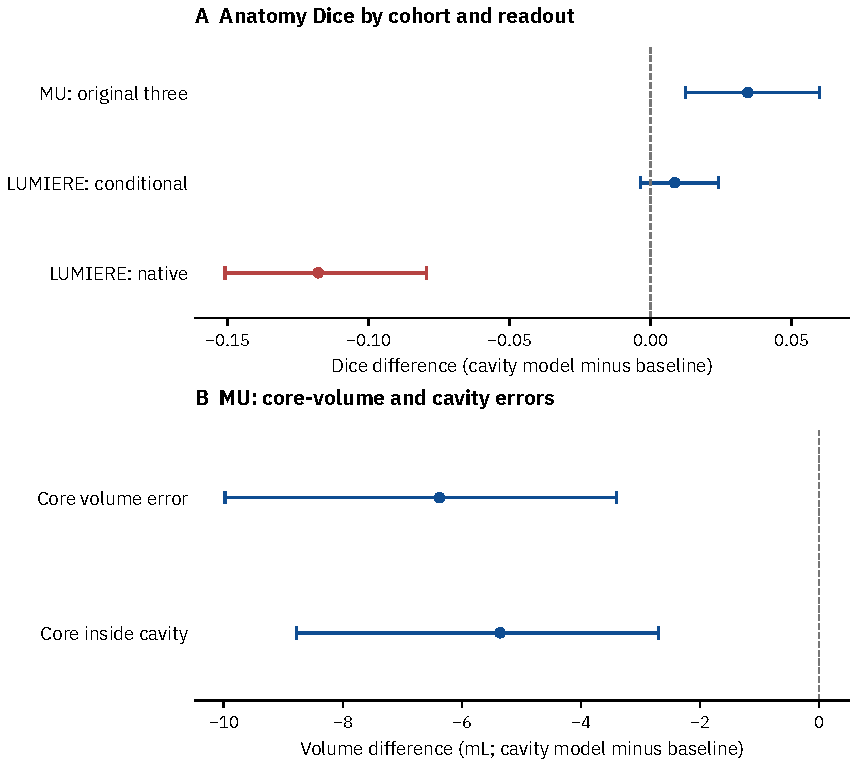
\includegraphics[width=\linewidth]{figures/updated_cavity.pdf}
\caption[Cavity supervision and readout effects]{Cavity-model changes relative to the preserved observation baseline. Panel A scores the original three lesion compartments: positive Dice differences favor the cavity model. Conditional LUMIERE scoring removes the cavity logit; native scoring keeps it. Panel B shows MU volume changes, where negative values favor the cavity model. Bars are unadjusted 95\% paired patient-bootstrap intervals from 4,000 draws. MU has 106 visits from 32 patients; LUMIERE has 178 visits from 18. All are reused selection data.}\label{fig:cavity}
\end{figure}

On LUMIERE, conditional four-category lesion Dice changed from 0.71045 to 0.71904, while the native five-category output scored 0.59256. The latter difference was -0.11789 [-0.15097, -0.07964]. LUMIERE has no cavity references; the native score measures agreement with its available labels. Missing-FLAIR lesion MAE increased from 0.57373 to 0.59040, a paired difference of +0.01667 [0.00458, 0.02658]. The MU improvement therefore comes with a cross-dataset and cross-task tradeoff: the native LUMIERE readout agrees less well with its available anatomical labels, and missing-FLAIR error rises.

\section{Completing missing MRI}

Completing current FLAIR tests information that the available sequences and their representation retain about an unobserved image. We compare CT1 alone, CT1 plus T1, and CT1 plus T1 plus T2 using three matched seeds and 116 visits from 18 LUMIERE patients; 112 visits contribute lesion scores. Lesion MAE fell from 0.90614 to 0.85781 after adding T1, then to 0.59294 after adding T2. The respective reductions were 5.33\% and 30.88\%. All four primary intervals, covering lesion and whole-brain error for both additions, favored the added sequence after multiplicity adjustment. T2 improved both endpoints in every scoring patient after seed averaging.

The decoder also needs access to useful spatial detail. A separate comparison enables or zeros its higher-resolution feature path. Enabling that path reduced lesion MAE from 0.75641 to 0.63469 and lesion-band gradient error from 0.23161 to 0.20923. All three seeds favored spatial access on lesion, gradient and nonlesion error. The paired lesion reduction was 0.12172 [0.08854, 0.14897], or 16.09\% of the zeroed arm's error. The direct-image sequence-addition reference scores 0.59294 on the same lesion endpoint. The 16.09\% reduction belongs to the spatial-path comparison; it is not a further reduction from the sequence-addition model. Figure~\ref{fig:completion} keeps these two comparisons separate.

\begin{figure}[htbp]\centering
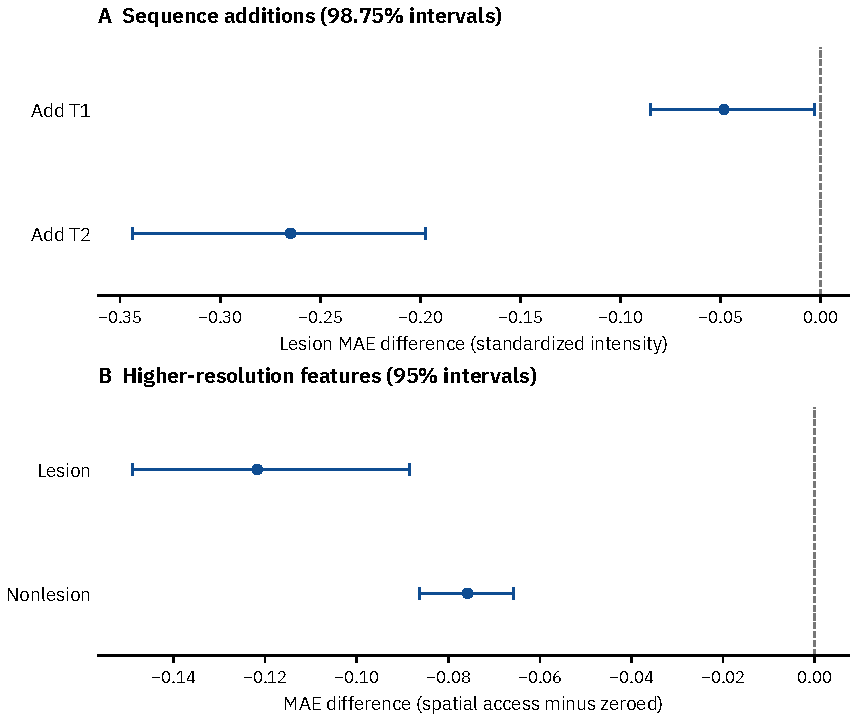
\includegraphics[width=\linewidth]{figures/updated_completion.pdf}
\caption[Sequence additions and spatial access]{FLAIR completion on reused LUMIERE development patients. Negative differences favor the added input or enabled spatial path. Panel A shows adjusted 98.75\% paired patient-bootstrap intervals from the sequence-addition study; panel B shows 95\% intervals from the spatial-feature study. Each comparison averages three seed scores over 18 patients. Lesion scoring uses 112 visits; nonlesion scoring uses 116. The two panels have independent scales.}\label{fig:completion}
\end{figure}

The compact state does not preserve all of the full predictor's completion performance. With new readouts fitted to frozen compact states, lesion MAE was 1.01734 for the enabled encoder's compact state and 0.74812 for the zeroed encoder's state; the full spatial-feature predictor scored 0.63469. The frozen-state segmentation study then reused the full learned state for segmentation on 116 visits from 18 patients, averaging three seeds. Its frozen learned features improved Dice over frozen random features by 0.06679 [0.05128, 0.08271]. Direct-image adaptation scored 0.07915 higher than the frozen learned state, with a paired 95\% difference interval of [0.06587, 0.09343]. That deficit exceeded the allowed 0.05 margin. The full representation occupies 334.75 MiB per visit, 4.05 times the Float32 input payload. Its learned features are useful, but retaining them has a substantial storage cost and still leaves a gap to direct-image adaptation.

\section{Forecasting anatomical measurements}\label{sec:initial-results}

Forecasting depends on both the current anatomical estimate and the prediction of its change. In the representation-forecast comparison, current-scan, mean-history and JEPA next-visit volume-error ratios relative to measured persistence were 1.325, 1.377 and 1.393 on LUMIERE. On SAILOR they were 3.374, 5.235 and 2.883. MRI models estimate anatomy from images, whereas persistence receives current mask measurements. These ratios therefore include the cost of estimating the current state. The matched history comparisons below test the additional value of earlier visits.

The frozen-history study compared history with latest-only MRI using the same past timing and availability information. On 75 pairs from 18 LUMIERE patients, history minus latest-only CRPS was +0.003 log1p(mm³), with an adjusted 99\% interval of [-0.047, +0.052]. The joint-training study allowed forecast gradients into the encoder; current-state MAE rose from 1.473 to 1.540 in the history arm. The supplied-horizon study provided the realized follow-up interval and obtained a 0.05\% history CRPS reduction, below its fixed 5\% criterion.

Adding recorded treatment status to MRI history gives a further test of the available context, using 242 SAILOR pairs from 27 patients. The CRPS difference was +0.001 [-0.081, +0.082], using a 99\% patient-bootstrap interval. The input was a coarse per-session status category whose prospective availability was unverified.

Supplying measured current anatomy removes the encoder's estimation error from the numerical forecast. With the retrospective interval also supplied, current-only CRPS was 1.007 against persistence at 1.120 on 253 pairs from 48 LUMIERE patients. The paired difference was -0.113 [-0.196, -0.031], using an adjusted 97.5\% interval. History reduced the point score by another 2.21\%, with an interval spanning zero. Transferred unchanged to 215 SAILOR pairs from 27 patients, current-only scored 1.020 against persistence at 0.867.

The regional regressions make the same question more spatially specific, using the source-volume measurements verified in Chapter~\ref{ch:testing}. Table~\ref{tab:regional} gives their errors on LUMIERE and MU. History reduced current-only error by 0.28\% on LUMIERE and about 0.046\% on MU. History error exceeded persistence by 2.68\% on LUMIERE and 10.07\% on MU; both adjusted paired intervals favored persistence. Both cohorts selected the strongest ridge penalty and a zero trend-extrapolation coefficient.

\begin{table}[htbp]\centering\small
\caption[Corrected regional-volume forecasts]{Regional MAE in log1p(mL), with patients weighted equally. LUMIERE uses three automated compartments; MU uses four reviewed compartments, including cavity.}\label{tab:regional}
\begin{tabular}{lrr}\toprule
 & LUMIERE & MU\\\midrule
Scored pairs or triples & 30 & 33\\
Patients & 8 & 18\\
Persistence & 0.281 & 0.16587\\
Current-only ridge & 0.289 & 0.18265\\
History ridge & 0.288 & 0.18256\\\bottomrule
\end{tabular}
\end{table}
\FloatBarrier

In MU, history lowers nonempty-cell MAE from 0.510 to 0.482 and raises empty-cell MAE from 0.012 to 0.047. LUMIERE shows the same direction of tradeoff. The improvement on nonempty cells is offset by added error on empty cells, and the patient-averaged regional results still favor persistence.

\section{History in image prediction}

Better completion provides a useful test of whether current-image gains carry over to forecasting. Adapting the encoder for completion reduces current-FLAIR MAE from 0.520 to 0.505 on 60 visits from 13 patients. On 45 future-image pairs from ten patients, adapted history, latest-only and persistence MAE were 0.656915, 0.656850 and 0.656362. Two-patient fitting and direct spatial-code fitting produced small improvements below their fixed fitting criteria. Smoothing persistence also reduced intensity MAE, showing how this metric can reward reduced image detail.

History-assisted completion asks whether an earlier scan helps even when the target is current FLAIR. This comparison uses 64 target visits from 18 patients and three seeds. Its intervals are paired 95\% patient bootstraps. Current-only, genuine-history and timing-matched donor-history lesion MAE were 0.56018, 0.57021 and 0.56843. Genuine history increased gradient error by 0.00318 [0.00051, 0.00573] against current-only and by 0.00398 [0.00120, 0.00662] against donor history. The learned models all beat registered previous-FLAIR persistence. The current-image control accounted for that advantage, while genuine history produced worse local gradients.

\section{Structured forecasts at 12 and 24 weeks}

Structured forecasts predict anatomical scenarios at requested horizons, allowing shape and volume to be assessed from the same outputs. The evaluation contains 259 targets: 112 and 89 LUMIERE targets at 12 and 24 weeks, and 36 and 22 MU targets. Figure~\ref{fig:structured} compares the segmentation scores and isolates the contribution of history.

\begin{figure}[htbp]\centering
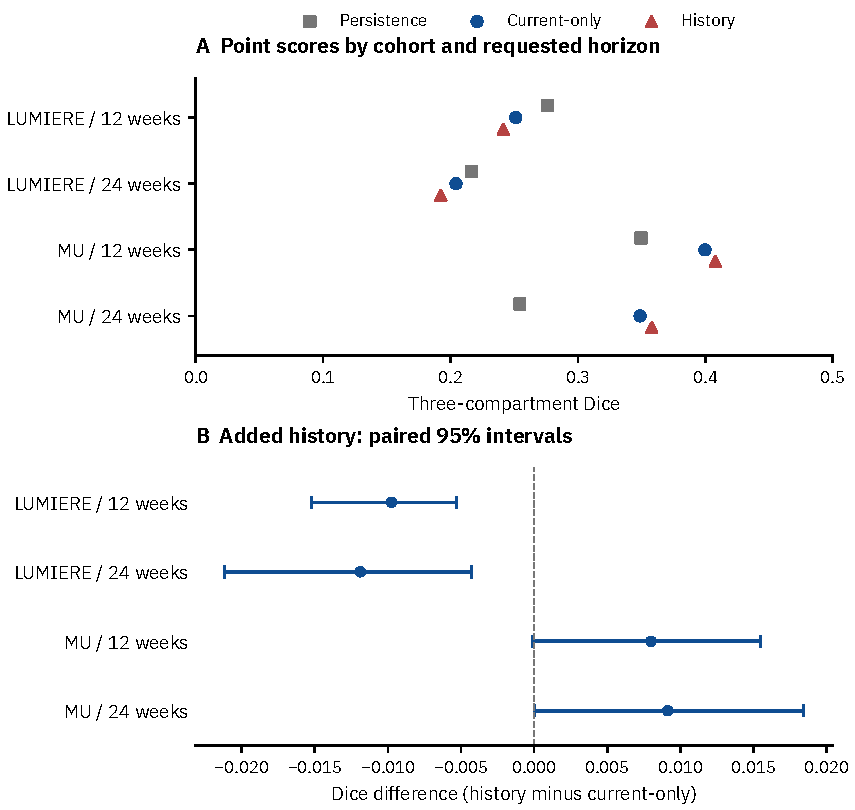
\includegraphics[width=\linewidth]{figures/updated_forecast.pdf}
\caption[Structured forecasts and added history]{Structured forecast Dice on reused selection patients. Higher is better. Panel A shows point scores for the weighted scenario-vote maps. Panel B shows history minus current-only with unadjusted 95\% paired patient-bootstrap intervals. LUMIERE has 112 targets/16 patients at 12 weeks and 89/15 at 24; MU has 36/18 and 22/13. Patients can contribute at both horizons.}\label{fig:structured}
\end{figure}
\FloatBarrier

History lowered Dice relative to current-only by 0.00975 on LUMIERE at 12 weeks and 0.01188 at 24 weeks, with both paired intervals below zero. MU differences were +0.00800 [-0.00010, +0.01551] and +0.00914 [+0.00004, +0.01844]. History had higher volume MAE in every cohort/horizon group. Its volume-CRPS contrasts with current-only and scalar-history controls all had intervals spanning zero.

The MU Dice gains over persistence were largely due to empty core compartments. At 24 weeks, current-only gained 9.44 percentage points overall; future-empty core contributed +10.26 points and nonempty core contributed -0.80 points under the original aggregate weights. Five of ten empty-core targets were correctly predicted empty. Three were resolutions from current reference volumes of 0.020, 0.045 and 0.662 mL; two were already empty. On the twelve targets whose core remained present, current-only Dice was 0.0422 below persistence, with a 95\% interval of [-0.0876, -0.0048].

Figure~\ref{fig:forecast-attribution} shows how the core strata and the other compartments contributed to the overall difference.
\begin{figure}[htbp]\centering
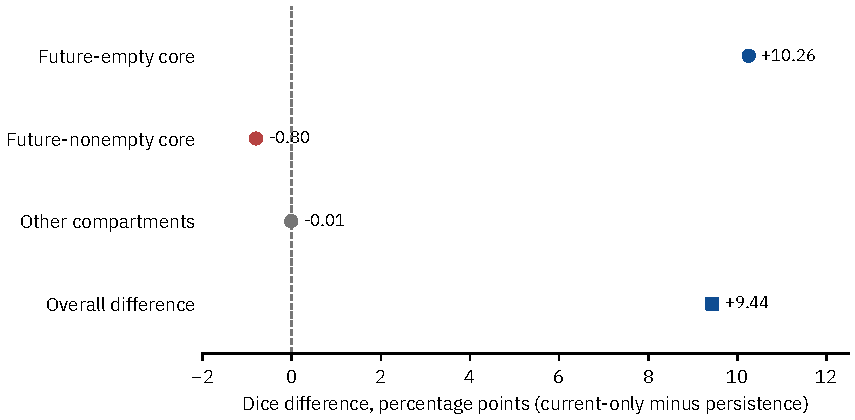
\includegraphics[width=\linewidth]{figures/updated_forecast_attribution.pdf}
\caption[Contributions to the MU 24-week forecast Dice difference]{Current-only minus model-persistence Dice on 22 MU 24-week targets from 13 reused selection patients. The first three points are contributions to the original patient-weighted, three-compartment aggregate, not within-group Dice differences. Other compartments combine compartments 1 and 3. The square is the overall difference. Values are in percentage points; points are descriptive estimates without intervals. Rounded contributions may not sum exactly to the rounded overall difference.}\label{fig:forecast-attribution}
\end{figure}

FLAIR abnormality showed a smaller gain across all 22 MU 24-week targets, each with a nonempty reference. Current-only improved Dice by 0.01264 [0.00414, 0.02144] over model persistence. Among 17 persistently nonempty targets from twelve patients whose reference volume changed by more than the larger of 2 mL or 20\% of its current value, the gain was 0.01456 [0.00547, 0.02439]. This supports a specific current-only gain in FLAIR-abnormality segmentation. It is a post-hoc development finding on 22 targets and requires independent confirmation.

Using the cavity-supervised observation state gives another current-only forecast comparison. At 24 weeks, original-three-compartment Dice increased from persistence's 0.2488 to 0.3760, while nonempty-core Dice fell from 0.1361 to 0.0123. Four-compartment volume CRPS improved from 16.4198 to 13.5597 mL; the scalar control scored 13.6599. Nonempty-core nominal 90\% coverage was 6.7\% at 12 weeks and 0\% at 24 weeks. The scalar control covered 93.3\% and 100\%, with wider intervals. The aggregate Dice gain therefore does not establish reliable recovery of nonempty core or calibrated uncertainty about its amount.

\section{Predicting compartment quantities}

The volume and coverage results motivate separating compartment presence and amount from spatial allocation. For the logistic quantity model, the 64-sample mean had 24-week nonempty-core MAE of 0.819 mL, compared with persistence at 1.281. Its exact fitted-distribution mean scored 1.769 mL. The corresponding Gaussian values were 1.475 and 1.691 mL. A small sample from these heavy-tailed distributions changed the apparent ranking. Deterministic CRPS was about 1.95--1.96 mL for both families at 24 weeks, against the frozen scalar control at 1.370.

Varying the fitting population and the available current and historical information gives 24 fits for comparison. The model receiving current MRI, history metadata, previous volumes and rates, and previous MRI had nonempty-core CRPS of 1.646 and 1.201 mL at 12 and 24 weeks, averaged across three seeds. Mean-volume MAE was 1.819 and 1.385 mL against persistence at 1.692 and 1.281. Nominal 90\% core coverage fell to 30.4\% and 25.0\%. No configuration met the required volume-error and CRPS conditions at both horizons under both the preselected seed and the average across three seeds.

Regularized scalar and PCA-MRI models use 156 fitting pairs from 56 patients and the same 58 selection targets. At 24 weeks, exact nonempty-core mean MAE was 11.065 mL for scalar inputs and 13.662 for added MRI components; CRPS was 2.571 and 2.686 mL. Both exceeded their persistence and scalar-distribution controls. Neither provides a satisfactory quantity model for spatial allocation: at each horizon, nonempty-core mean-volume MAE must be no worse than persistence and CRPS no worse than the scalar-distribution control. Neither model meets both conditions.

\section{Choosing MRI sequences}

The acquisition comparison tests whether predicted candidate features help choose the next sequence, using 48 MU visits from 16 development patients. Fixed, direct and JEPA policies chose the same path on every visit: T1, then CT1, then FLAIR. All score 0.62525 on anatomy utility averaged after observing two and three sequences. Identical choices leave no observed advantage for either learned policy. Oracle utility was 0.62709, a gain of 0.00184 [0.00010, 0.00410] under this observer and offline reveal task.

Missing-FLAIR completion improved against the preserved cavity-aware reference on every fixed input panel (Figure~\ref{fig:acquisition}). With T1, CT1 and T2 available, lesion MAE fell from 0.5879 to 0.5270. All four paired intervals favor the new observer, and every panel remains within the +0.05 retention allowance.

All-four-sequence anatomy Dice fell from 0.71769 to 0.67177, a difference of -0.04592 [-0.07020, -0.02220]. The interval crossed the -0.05 retention margin. Empty-core false-positive volume increased from 1.179 to 1.976 mL, and empty-cavity false positives increased from 4.516 to 8.908 mL. The observer improves completion while reducing anatomical agreement, so the gain depends on which readout is used. Its full four-sequence state occupies 16.09 GB; encoding averaged 12.84 seconds and the shared anatomy/image readout 1.58 seconds. These costs also limit its practicality as a patient state.

\FloatBarrier
\begin{figure}[htbp]\centering
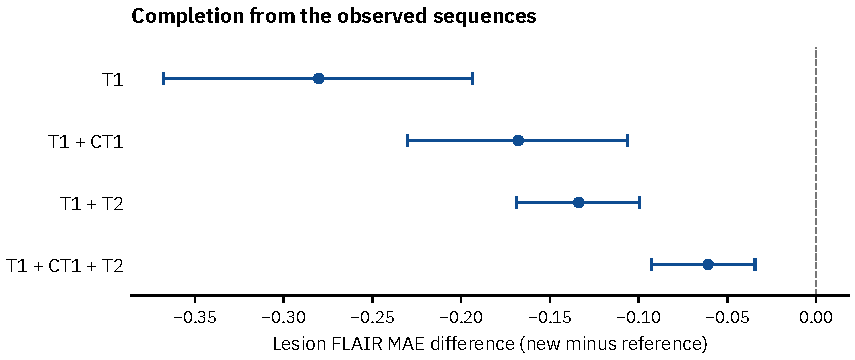
\includegraphics[width=\linewidth]{figures/updated_acquisition.pdf}
\caption[Missing-FLAIR completion in the acquisition study]{Lesion-region MAE differences in standardized intensity units on 48 MU visits from 16 development patients. Negative values favor the acquisition observer. Bars are paired 95\% patient-bootstrap intervals. The reference observer was trained on a broader population.}\label{fig:acquisition}
\end{figure}

\section{What predictive learning retains}

The preceding results judge representations through anatomical and image outputs. A clinical-classification comparison also tests whether the predictive objective adds useful information beyond direct adaptation, scoring ten patients. Calibrated log loss was 0.80850 for adapted direct BrainIAC, 0.81117 for proper JEPA and 0.81778 for shuffled-target JEPA; the fitting-prevalence control scored 0.70880. Proper JEPA was slightly worse than direct in both seeds. All declared objective contrasts had adjusted intervals spanning zero, providing no clear incremental benefit from the tested JEPA objective.

The shape-and-activity simulator makes the distinction between retained factors explicit. Predictive representations recover ellipse axes with normalized mean-squared error near 0.02, while the local activity factor remains poorly recovered, with a Brier score near 0.25. Direct factor supervision achieves activity Brier 0.10890 and 85.35\% accuracy. In this controlled setting, good recovery of global shape coexists with poor recovery of a local factor. A predictive objective alone does not ensure that a readout can recover every quantity needed for a downstream task.

\endgroup

\clearpage
\chapter{Conclusion}
\begingroup
\clubpenalty=10000
\makeatletter\@clubpenalty=10000\makeatother
\widowpenalty=10000
\brokenpenalty=10000

We set out to learn a patient state that describes current anatomy and uses earlier MRI to predict future anatomy. The results give stronger support to current-state estimation. Mask supervision improves volume estimates, additional sequences improve FLAIR completion, and higher-resolution features preserve detail lost by compact states. Explicit cavity supervision also reduces confusion between postoperative cavity and core.

These improvements do not consistently carry over to forecasting. Earlier MRI provides no established practical gain over matched current-only models in the tested cohorts. Regional forecasts favor persistence on LUMIERE and MU. Measured anatomy and retrospective timing improve LUMIERE forecasts, but this advantage does not transfer to SAILOR. Completion adaptation likewise improves current FLAIR without improving its forecast.

The structured model gives a narrower positive result: current-only MU FLAIR-abnormality Dice improves by 0.01264 over persistence at 24 weeks on 22 development targets. Most of the larger aggregate Dice gain comes from empty core compartments, and volume-distribution performance remains weaker. The positive claim is specific to the FLAIR segmentation endpoint and requires independent confirmation.

For acquisition, fixed and learned policies select the same sequence order. The observer improves missing-FLAIR completion while reducing all-sequence anatomical agreement. A state intended for several tasks therefore needs to be assessed through each readout.

MRI results come from reused development cohorts. Patient-level partitions separate fitting and scoring, but subsequent model choices draw on earlier results. LUMIERE and SAILOR use automated anatomical references; MU provides reviewed per-scan masks without independent longitudinal adjudication. Clinical interpretation also requires treatment context verified at the prediction cutoff. The work supports useful anatomical and completion representations, while a reliable, transferable benefit from patient history remains unestablished.

\endgroup

\clearpage\phantomsection\addcontentsline{toc}{chapter}{REFERENCES}\markboth{References}{}\begin{singlespace}\begin{thebibliography}{99}
\interlinepenalty=10000

\bibitem{ref1} P. Y. Wen et al., “RANO 2.0: Update to the Response Assessment in Neuro-Oncology criteria for high- and low-grade gliomas in adults,” Journal of Clinical Oncology, vol. 41, no. 33, pp. 5187–5199, 2023, doi: 10.1200/JCO.23.01059.

\bibitem{ref2} M. A. Qazi, M. Nadeem, and M. Yaqub, “Beyond generative AI: World models for clinical prediction, counterfactuals, and planning,” arXiv preprint arXiv:2511.16333, 2025, doi: 10.48550/arXiv.2511.16333.

\bibitem{ref3} M. Assran et al., “Self-supervised learning from images with a joint-embedding predictive architecture,” in Proc. IEEE/CVF Conference on Computer Vision and Pattern Recognition, 2023, pp. 15619–15629, doi: 10.1109/CVPR52729.2023.01499.

\bibitem{ref4} Y. Suter et al., “The LUMIERE dataset: Longitudinal Glioblastoma MRI with expert RANO evaluation,” Scientific Data, vol. 9, art. 768, 2022, doi: 10.1038/s41597-022-01881-7.

\bibitem{ref5} Y. Yang et al., “Medical world model,” in Proc. IEEE/CVF International Conference on Computer Vision, 2025, pp. 8319–8329, doi: 10.1109/ICCV51701.2025.00779.

\bibitem{ref6} V. Biller et al., “TumorFlow: Physics-guided longitudinal MRI synthesis of glioblastoma growth,” arXiv preprint arXiv:2603.04058, 2026, doi: 10.48550/arXiv.2603.04058.

\bibitem{ref7} Q. Liu et al., “Treatment-aware diffusion probabilistic model for longitudinal MRI generation and diffuse glioma growth prediction,” IEEE Transactions on Medical Imaging, vol. 44, no. 6, pp. 2449–2462, 2025, doi: 10.1109/TMI.2025.3533038.

\bibitem{ref8} D. Laslo et al., “Generative AI for spatial tumor growth on MRI: A proof-of-principle study in pediatric diffuse midline glioma,” BMC Medicine, vol. 24, art. 389, 2026, doi: 10.1186/s12916-026-04911-y.

\bibitem{ref9} S. Huisman, N. Belkacemi, V. C. Keil, J. Verhoeff, and S. David, “Rectified flow-based prediction of post-treatment brain MRI from pre-radiotherapy priors for patients with glioma,” arXiv preprint \href{https://arxiv.org/abs/2603.08385v2}{arXiv:2603.08385v2}, 2026, doi: 10.48550/arXiv.2603.08385.

\bibitem{ref10} Y. Yue, Y. Wang, C. Tao, P. Liu, S. Song, and G. Huang, “CheXWorld: Exploring image world modeling for radiograph representation learning,” in Proc. IEEE/CVF Conference on Computer Vision and Pattern Recognition, 2025, pp. 20778–20788.

\bibitem{ref11} H. Huang et al., “Learning sparse latent predictive foundation model for multimodal neuroimaging,” arXiv preprint \href{https://arxiv.org/abs/2606.14957v5}{arXiv:2606.14957v5}, 2026, doi: 10.48550/arXiv.2606.14957.

\bibitem{ref12} F. Mager and L. K. Hansen, “Contrastive joint-embedding prediction for representation learning in structural MRI,” arXiv preprint arXiv:2607.11962, 2026, doi: 10.48550/arXiv.2607.11962.

\bibitem{ref13} T. Z. Li et al., “Self-supervised learning of imaging and clinical signatures using a multimodal joint-embedding predictive architecture,” arXiv preprint arXiv:2509.15470, 2025, doi: 10.48550/arXiv.2509.15470.

\bibitem{ref14} J. Bai and J. Xiong, “Temporal-distance JEPA: Plan-aware representation learning for latent world model predictive control,” arXiv preprint arXiv:2607.25337, 2026, doi: 10.48550/arXiv.2607.25337.

\bibitem{ref15} L. Chen, N. Zebardast, M. Wang, T. Elze, and J. I. Comander, “Training-inference input alignment outweighs framework choice in longitudinal retinal image prediction,” arXiv preprint \href{https://arxiv.org/abs/2604.16955v1}{arXiv:2604.16955v1}, 2026, doi: 10.48550/arXiv.2604.16955.

\bibitem{ref16} D. Tak et al., “A generalizable foundation model for analysis of human brain MRI,” Nature Neuroscience, vol. 29, pp. 945–956, 2026, doi: 10.1038/s41593-026-02202-6.

\bibitem{ref17} Y. Suter et al., “LUMIERE dataset: MRI data and automated segmentations,” Figshare, version 1, 2022, data set, doi: 10.6084/m9.figshare.21249516.v1.

\bibitem{ref18} I. T. Hovden et al., “Brain tumor MRI: Serial assessments in longitudinal oncological research (SAILOR),” EBRAINS, version 1, 2023, data set, doi: 10.25493/D948-J3P.

\bibitem{ref19} D. Yaseen et al., “University of Missouri Post-operative Glioma Dataset (MU-Glioma-Post),” The Cancer Imaging Archive, version 1, 2025, data set, doi: 10.7937/7K9K-3C83.
\bibitem{record} Project research record, ``Experiments and evidence'' and ``Methods,'' evidence through November 9, 2026; ``Final study synthesis,'' closed November 11, 2026. Repository records: \texttt{info/EXPERIMENTS.md}, \texttt{info/METHODS.md}, and \texttt{info/STUDY\_SUMMARY.md}. Figure aggregates and source hashes accompany this report.
\end{thebibliography}\end{singlespace}
\end{document}
